\documentclass[12pt,a4paper,onecolumn]{article}
\usepackage[utf8]{inputenc}
\usepackage[T1]{fontenc}
\usepackage[french]{babel}
\usepackage{amsmath}
\usepackage{amsfonts}
\usepackage{amssymb}
\usepackage{amscd}
\usepackage{amsthm}
\usepackage{physics}
\usepackage[left=2.2cm,right=2.2cm,top=2cm,bottom=2cm]{geometry}
\usepackage{textcomp,gensymb} %pour le °C, et textcomp pour éviter les warning
\usepackage{graphicx} %pour les images
\usepackage{subcaption}
\usepackage[colorlinks=true,breaklinks=true,
	citecolor=blue,
	linkcolor=blue,
	urlcolor=blue]{hyperref} % pour insérer des liens
\usepackage{epstopdf} %converting to PDF
\usepackage[export]{adjustbox} %for large figures

\usepackage{array}
\usepackage{dsfont}% indicatrice : \mathds{1}
%\usepackage[dvipsnames]{xcolor}

% ------------------------- Bilbiographie --------------------------------------
\usepackage[backend=biber]{biblatex}
\addbibresource{biblio.bib}
% ------------------------------------------------------------------------------

% ------------------------- Color table ----------------------------------------
\usepackage{multirow}
\usepackage[table]{xcolor}
\definecolor{maroon}{cmyk}{0,0.87,0.68,0.32}
% ------------------------------------------------------------------------------

\setcounter{tocdepth}{4} %Count paragraph
\setcounter{secnumdepth}{4} %Count paragraph
\usepackage{float}

\usepackage{graphicx} % for graphicspath
\graphicspath{{../images/}}

\usepackage{array,tabularx}
\newcolumntype{L}[1]{>{\raggedright\let\newline\\\arraybackslash\hspace{0pt}}m{#1}}
\newcolumntype{C}[1]{>{\centering\let\newline\\\arraybackslash\hspace{0pt}}m{#1}}
\newcolumntype{R}[1]{>{\raggedleft\let\newline\\\arraybackslash\hspace{0pt}}m{#1}}

\title{Etude du premier modèle de Hindmarsh-Rose}
\author{Vincent Matthys Maureen Muscat Mariène Wan}


\renewcommand{\thesubsection}{\alph{subsection}}


\begin{document}
%\maketitle
\begin{tabularx}{\textwidth}{@{} l X r @{} }
{\textsc{Master Bio Informatique et Modélisation}} & & Rapport de Projet \\
UE MMCN & &{Université Pierre et Marie Curie}\\
%& %M1 Informatique
\end{tabularx}
\vspace{1.5cm}
\begin{center}

\rule[11pt]{5cm}{0.5pt}

\textbf{\LARGE \textsc{\'Etude du premier modèle de Hindmarsh-Rose}}
\vspace{0.5cm}

Vincent Matthys, Maureen Muscat et Mariène Wan


\rule{5cm}{0.5pt}

\vspace{1.5cm}


\begin{figure}[ht]
\begin{center}
\includegraphics[angle=270, origin =c, width = 0.9\textwidth]{1.eps}
\end{center}
\caption{Plan de phase, avec les nullclines en couleurs et une solution en noir avec I = 2 et c = 2}
\end{figure}

\end{center}


%\href{https://github.com/VincentMatthys/Hindmarsh_Rose.git}{Lien github}\\
\href{https://tel.archives-ouvertes.fr/tel-00453912v1/document}{Etude du  modèle Hindmarsh-Rose}


\newpage
\tableofcontents

\newpage

\section{Etude théorique}


\begin{equation}
\left\{
\begin{array}{l l}
v'(t)= \displaystyle{\frac{w - v^3 + 3v^2 +I_{ap}}{c}} = f(v,w) & \text{ avec } c\neq 0\\
w'(t) = 1 - 5 v^2 - w = g(v,w) & \\
\end{array}
\right.
\end{equation}

\subsection{Recherche des nullclines}

Recherche des nullclines :
\begin{align*}
\text{Nullcline\,pour\,v : } v' &= 0  &\Leftrightarrow w &= v^3 - 3 v^2 - I_{ap}\\
\text{Nullcline\,pour\,w : } w' &= 0 &\Leftrightarrow w &= 1-5v^2
\end{align*}
La nullcline de $v$ est de forme \textbf{cubique}. \\
La nullcline de $w$ est une \textbf{parabole}.

Les \textbf{points stationnaires} sont les points à l'intersection des deux nullclines, c'est-à-dire les points dans le plan de phase dont le vecteur tangent a ses deux composantes nulles. Nous résolvons :

$$
v^3 - 3 v^2 - I_{ap} = 1-5v^2
$$
\begin{equation} \label{Stat}
v^3 + 2v^2 -I_{ap} -1 = 0
\end{equation}



\subsubsection{Résolution par la méthode de Cardan}
On peut réecrire \ref{Stat} sous la forme suivante :
\begin{equation*}
av^3 + b v^2 + cv + d = 0
\end{equation*}

Où $a = 1$, $b = 2$, $c = 0$ et $d = -(I_{ap} + 1)$.
Et d'après la méthode de Cardan, le changement de variable se fait selon la formule : $$ v=t-\frac{b}{3a} $$

On pose alors $v = t - \frac{2}{3}$ et on obtient l'équation suivante :

\begin{align}
\left(t - \frac{2}{3}\right)\left(t^2 - \frac{4}{3}t + \frac{4}{9}\right) + 2t^2 - \frac{8}{3}t + \frac{8}{9} - 1 - I_{ap} &= 0 \nonumber\\
t^3 - 2t^2 + \frac{4}{9}t + \frac{8}{9}t - \frac{8}{27} +2t^2 - \frac{8}{3}t + \frac{8}{9} - 1 - I_{ap} &= 0 \nonumber\\
t^3 - \frac{4}{3}t - \frac{11}{27} - I_{ap} &= 0 \label{eqCadran}
\end{align}

On peut alors résoudre l'équation \ref{eqCadran} par la méthode de Cardan :

\begin{align}
\Delta_1 &= -\left(-\left(\frac{11}{27} + I_{ap}\right)\right)^2 - \frac{4}{27}\left(-\frac{4}{3}\right)^3 \nonumber\\
\Delta_1 &= -\frac{121}{729} - \frac{22}{27}I_{ap} - I_{ap}^2 + \frac{4}{27}\frac{64}{27} \nonumber\\
\Delta_1 &= -I_{ap}^2 - \frac{22}{27}I_{ap} + \frac{5}{27} \nonumber\\
\Delta_1 &= -(I_{ap} + 1)(I_{ap} - \frac{5}{27})
\end{align}

\newpage

Suivant cette méthode :
\begin{itemize}
\item Si $\Delta_1 > 0$, alors il y a trois solutions réelles distinctes.
\item Si $\Delta_1 = 0$, alors il y a deux solutions réelles dont une solution double.
\item Si $\Delta_1 < 0$, alors une solution est réelle et les deux autres sont complexes conjuguées.
\end{itemize}
On utilisera à profit la notation trigonométrique des solutions réelles telle que présentée par la littérature.

\paragraph{$\Delta_1 > 0$} L'équation possède trois solutions réelles distinctes.


En repartant de \ref{eqCadran}, et en posant $t = u\cos(\theta)$ il vient :
\begin{equation}
u^3\cos^3(\theta) -\frac{4}{3}u\cos(\theta)-\left(\frac{11}{27} + I_{ap}\right) = 0
\label{equcos}
\end{equation}
L'idée est de choisir $u$ pour se ramener à la relation :
$ 4\cos^3(\theta) - 3\cos(\theta)-\cos(3\theta) = 0 $, démontrée ci-après :

\begin{align*}
  \cos(3\theta)
  &= \cos(2\theta + \theta)\\
  &= \cos(2\theta)\cos(\theta) - \sin(2\theta)\sin(\theta) \\
  &= (2\cos^2(\theta) - 1)\cos(\theta) - 2\sin(\theta)\cos(\theta)\sin(\theta)\\
  &= 2\cos^3(\theta) - \cos(\theta) - 2\cos(\theta)(1-\cos^2(\theta))\\
  &= 2\cos^3(\theta) - \cos(\theta) - 2\cos(\theta) + 2\cos^3(\theta)\\
  &= 4\cos^3(\theta) - 3\cos(\theta) \qedhere
\end{align*}

En divisant \ref{equcos} par $u^3$ puis en posant $u = \frac{4}{3}$ :
\begin{align*}
\cos^3(\theta) - \frac{\left(\frac{4}{3}\right)^2}{\left(\frac{4}{3}\right)^3}\cos(\theta)-\frac{\frac{11}{27} + I_{ap}}{\left(\frac{4}{3}\right)^3} &= 0 \\
\cos^3(\theta) - \frac{3}{4}\cos(\theta) - \frac{\frac{11}{27} + I_{ap}}{\left(\frac{4}{3}\right)^3}&= 0 \\
4\cos^3(\theta) - 3\cos(\theta) - \frac{27}{16}\left(\frac{11}{27} + I_{ap}\right)&= 0 \tag*{en multipliant par 4}
\end{align*}

On reconnaît alors l'identité trigonométrique souhaitée et il reste :
\begin{equation}
\cos(3\theta) = \frac{11 + 27I_{ap}}{16} \label{eqtheta}
\end{equation}

Or étant dans le cas $\Delta_1 > 0$, on a $-1 < I_{ap} < \frac{5}{27}$, donc $-1 < \frac{11 + 27I_{ap}}{16} < 1$.
On peut donc résoudre \ref{eqtheta} sur un intervalle de $2\pi$ à l'aide de $\arccos$ et on a 3 solutions :

\begin{alignat*}{2}
&\theta_1 &&= \frac{1}{3}\arccos(\frac{11 + 27I_{ap}}{16})\\
&\theta_2 &&= \frac{1}{3}\arccos(\frac{11 + 27I_{ap}}{16}) + \frac{2\pi}{3}\\
&\theta_3 &&= \frac{1}{3}\arccos(\frac{11 + 27I_{ap}}{16}) + \frac{4\pi}{3}
\end{alignat*}

En remontant à l'expression des $t$ correspondant, il vient :

\begin{alignat*}{3}
&t_1 &&= u\cos(\theta_1) &&= \frac{4}{3}\cos(\frac{1}{3}\arccos(\frac{11 + 27I_{ap}}{16}))\\
&t_2 &&= u\cos(\theta_1) &&= \frac{4}{3}\cos(\frac{1}{3}\arccos(\frac{11 + 27I_{ap}}{16}) + \frac{2\pi}{3})\\
&t_3 &&= u\cos(\theta_1) &&= \frac{4}{3}\cos(\frac{1}{3}\arccos(\frac{11 + 27I_{ap}}{16}) + \frac{4\pi}{3})
\end{alignat*}

Soit les solutions en $v$ suivantes, en accord avec \cite{zwillinger2011crc} page 734:
\begin{alignat}{3}
&v_1 &&= t_1 - \frac{2}{3} &&= \displaystyle{\frac{2}{3}\left(2\cos\left(\frac{1}{3}\arccos\left(\frac{11 + 27I_{ap}}{16}\right)\right) - 1\right)} \label{Branche1}\\
&v_2 &&= t_2 - \frac{2}{3} &&= \displaystyle{\frac{2}{3}\left(2\cos\left(\frac{1}{3}\arccos\left(\frac{11 + 27I_{ap}}{16}\right) + \frac{2\pi}{3}\right) - 1\right)} \label{Branche2}\\
&v_3 &&= t_3 - \frac{2}{3} &&= \displaystyle{\frac{2}{3}\left(2\cos\left(\frac{1}{3}\arccos\left(\frac{11 + 27I_{ap}}{16}\right) + \frac{4\pi}{3}\right) - 1\right)} \label{Branche3}
\end{alignat}

\paragraph{$\Delta_1 = 0$} L'équation possède alors deux solutions réelles, une simple ($t_1$) et une double ($t_2$) :

$\left\{
\begin{array}{rl}
t_1 &= \displaystyle{\frac{3q}{p}}\\
t_2 &= \displaystyle{\frac{-3q}{2p}}\\
\end{array}
\right.$
avec :
$p = -\displaystyle{\frac{4}{3}}$ et $q = -\displaystyle{\left(\frac{11}{27} + I_{ap}\right)}$

Soit les solutions en $v$ suivantes :

\begin{alignat}{4}
&v_1 &&= t_1 - \frac{2}{3} &&= \displaystyle{\frac{-3(\frac{11}{27} + I_{ap})}{-\frac{4}{3}} - \frac{2}{3}} &&= \frac{9}{4}\left(\frac{1}{9} + I_{ap}\right) \\
&v_2 &&= t_2 - \frac{2}{3} &&= \displaystyle{\frac{3(\frac{11}{27} + I_{ap})}{-2\frac{4}{3}} - \frac{2}{3}} &&= -\frac{9}{8}\left(1 + I_{ap}\right)
\end{alignat}

\paragraph{$\Delta_1 < 0$} L'équation possède alors une solution réeelle et deux solutions complexes :
La solution réelle en $v$, d'après \cite{holmes200286}, avec $p = -\displaystyle{\frac{4}{3}}$ et $q = -\displaystyle{\left(\frac{11}{27} + I_{ap}\right)}$ :
\begin{align}
v_1 &= \displaystyle{-2\frac{\abs{q}}{q}\sqrt{-\frac{p}{3}}\cosh\left(\frac{1}{3}\cosh\left(-\frac{3q}{2p}\sqrt{-\frac{3}{p}}\right)\right)-\frac{2}{3}} \nonumber\\
&= \displaystyle{\frac{2}{3}\left(2\frac{\abs{-\left(\frac{11}{27} + I_{ap}\right)}}{\left(\frac{11}{27} + I_{ap}\right)}\cosh\left(\frac{1}{3}\cosh\left(\frac{27}{16}\abs{-\left(\frac{11}{27} + I_{ap}\right)}\right)\right) - 1\right)} \label{BrancheSolo}
\end{align}

\newpage
\subsubsection{Résultats}
L'équation \ref{Stat} à 1, 2 ou 3 solution selon la valeur de $I_{ap}$.




\begin{tabular}{|>{\centering\arraybackslash}m{3cm} | >{\centering\arraybackslash}m{3cm} |>{\centering\arraybackslash}m{3.5cm}  |c |}
\hline
Valeur de $I_{ap}$ & $\Delta_1$ & Nombre de points stationnaires & Nullclines \\
\hline
$I_{ap}< - 1$ &  $\Delta_1<0$ &  1 & \raisebox{-.5\height}{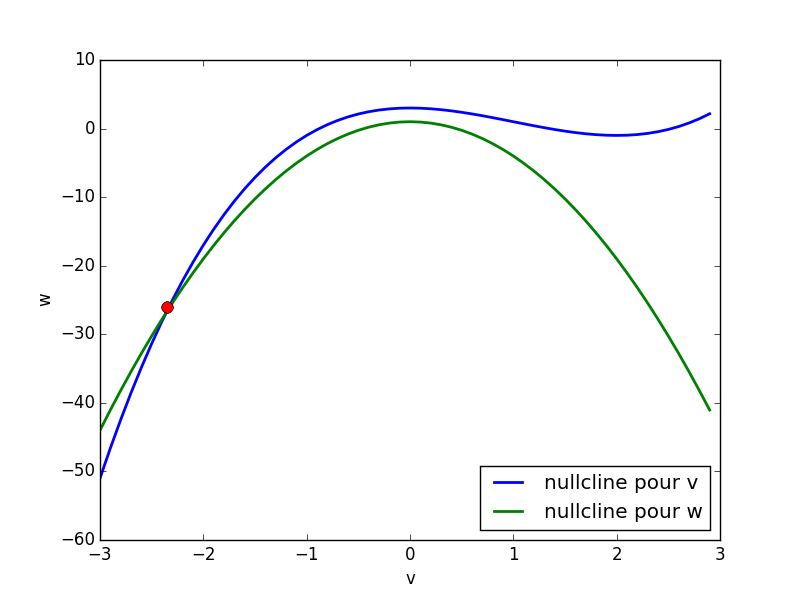
\includegraphics[height=0.27\linewidth]{tablestat1.png}} \\
  \hline
$I_{ap}= - 1$ &  $\Delta_1=0$ &  2 & \raisebox{-.5\height}{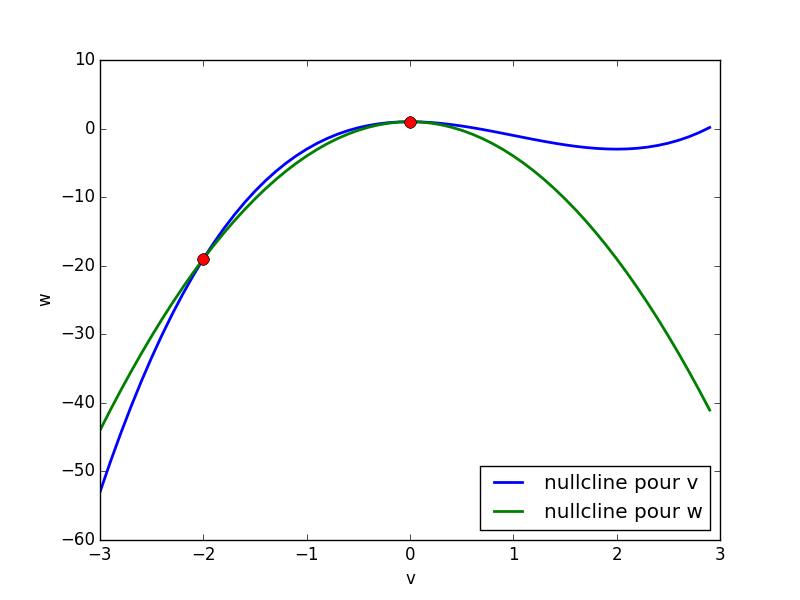
\includegraphics[height=0.27\linewidth]{tablestat2.png}} \\
  \hline
$-1<I_{ap}< 5/27$ &  $\Delta_1>0$ &  3 & \raisebox{-.5\height}{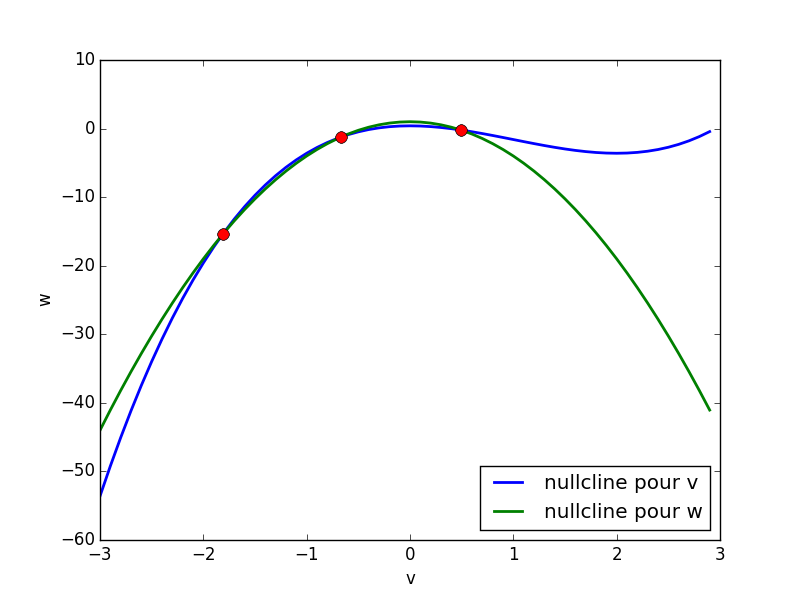
\includegraphics[height=0.27\linewidth]{tablestat3.png}} \\
  \hline
$I_{ap}=5/27$  &  $\Delta_1=0$ &  2 & \raisebox{-.5\height}{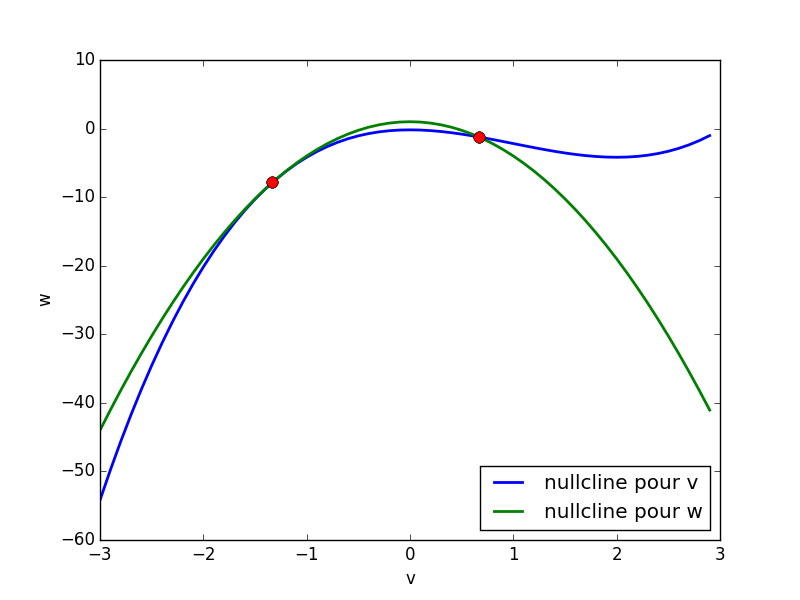
\includegraphics[height=0.27\linewidth]{tablestat4.png}} \\
  \hline
$I_{ap}> 5/27$ &  $\Delta_1<0$ &  1 & \raisebox{-.5\height}{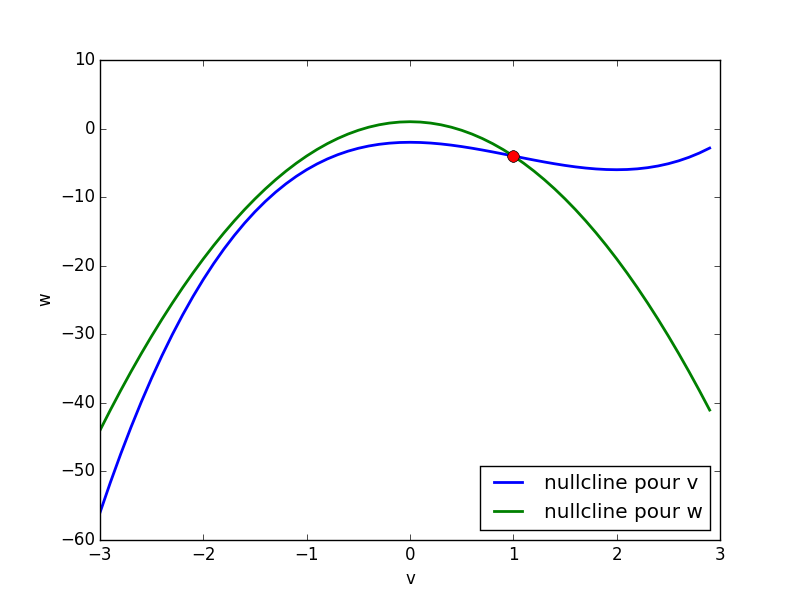
\includegraphics[height=0.27\linewidth]{tablestat5.png}} \\
 \hline
\end{tabular}


\begin{figure}[ht]
\begin{center}
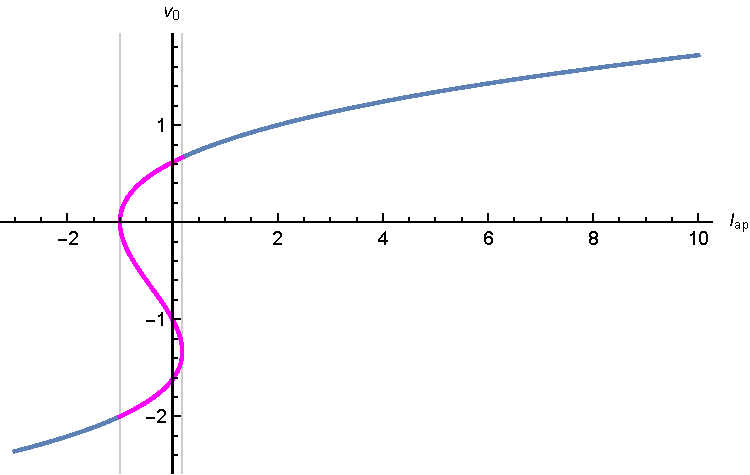
\includegraphics[origin =c, width = 0.9\textwidth]{Cardan}
\end{center}
\caption{Branches de points stationnaires par la méthode de Cardan}
\end{figure}



\subsection{Stabilité et bifurcations}
\subsubsection{Matrice Jacobienne du système}

\begin{equation*}
J(v,w)=
\begin{pmatrix}
\displaystyle{\frac{\partial f}{\partial v}(v,w)} & \displaystyle{\frac{\partial f}{\partial w}(v,w)} \\ \displaystyle{\frac{\partial g}{\partial w}(v,w)} & \displaystyle{\frac{\partial g}{\partial w}(v,w)}
\end{pmatrix}
=
\begin{pmatrix}
\displaystyle{\frac{-3v}{c}(v-2)} & \displaystyle{\frac{1}{c}} \\ -10v & -1
\end{pmatrix}
=J(v)
\end{equation*}


Matrice jacobienne en un point $(v_0 ; w_0)$

\begin{align*}
\det
\begin{pmatrix}
\displaystyle{\frac{-3v_0}{c}(v_0-2) -\lambda} & \displaystyle{\frac{1}{c}} \\ -10v_0 & -1 - \lambda
\end{pmatrix}
		&= \lambda^2 - Tr(J(v_0)) \lambda + \det(J(v_0)) \\
        &= \lambda^2 + \left(\frac{3v_0}{c}(v_0 - 2) + 1\right)\lambda + \frac{v_0}{c}(4 + 3 v_0)\\
        &= \lambda^2 + \left(\frac{3}{c}v_0^2-\frac{6}{c}v_0 + 1\right)\lambda + \left(\frac{3}{c}v_0^2 + \frac{4}{c}v_0\right)
\end{align*}

On distingue différents cas de stabilité en fonction du signe de $ \det(J(v_0))$ et de $Tr(J(v_0))$.

Le discriminant réduit de $Tr(J(v_0)) = 0$ est $\Delta' = \left(\frac{3}{c}\right)^2 - \frac{3}{c} = \frac{3}{c}(\frac{3}{c} - 1)$. Si $c < 3$ alors $\Delta' > 0$ et $Tr(J(v_0)) = 0$ admet deux racines réelles données par :

\begin{equation}
x_{Tr+} = \displaystyle{\frac{\frac{3}{c} + \sqrt{ \frac{3}{c}(\frac{3}{c} - 1)}}{\frac{3}{c}}} = \displaystyle{1 + \sqrt{1 - \frac{c}{3}}}\quad \text{et}\quad x_{Tr-} = \displaystyle{1 - \sqrt{1 - \frac{c}{3}}}
\label{TrJ}
\end{equation}

De plus $\det(J(v_0)) = \frac{v_0}{c}(3v_0 + 4) = 0$ admet 2 racines réelles :
\begin{equation}
x_{Det+} = 0 \quad \text{et} \quad x_{Det-} = \displaystyle{-\frac{4}{3}} \label{DetJ}
\end{equation}


\subsubsection{Expression des valeurs propres}

$$\Delta = \left(\frac{3v_0}{c}(v_0 - 2) + 1\right)^2 - 4\frac{v_0}{c}(4 + 3v_0) = \frac{9v_0^4}{c^2} - \frac{36v_0^3}{c^2} + \frac{6}{c}(\frac{6}{c} - 1)v_0^2 - \frac{28v_0}{c} + 1$$


$$
\begin{array}{l l}
\text{Pour }\Delta > 0 &\lambda_{\pm} = \frac{1}{2}\displaystyle{\left(-\left(\frac{3v_0}{c}(v_0 - 2) + 1\right) \pm \sqrt{\left(\frac{3v_0}{c}(v_0 - 2) + 1\right)^2-4\left(\frac{3}{c}v_0^2 + \frac{4}{c}v_0\right)}\right)} \\
 {\text{Pour }\Delta = 0} &\lambda_{\pm} = \frac{1}{2}\displaystyle{\left(\frac{3v_0}{c}(2 - v_0) - 1\right)} \\
{\text{Pour }\Delta < 0} &\lambda_{\pm} = \frac{1}{2}\displaystyle{\left(-\left(\frac{3v_0}{c}(v_0 - 2) + 1\right) \pm i\sqrt{4\left(\frac{3}{c}v_0^2 + \frac{4}{c}v_0\right) - \left(\frac{3v_0}{c}(v_0 - 2) + 1\right)^2}\right)} \\
\end{array}
$$


%\begin{align*}
%\lambda_{\pm} &= \frac{1}{2}\displaystyle{\left(-\left(\frac{3v_0}{c}(v_0 - 2) + 1\right) \pm \sqrt{\left(\frac{3v_0}{c}(v_0 - 2) + 1\right)^2-4\left(\frac{3}{c}v_0^2 + \frac{4}{c}v_0\right)}\right)}  \tag*{pour $\Delta > 0$}\\
%\lambda_{\pm} &= \frac{1}{2}\displaystyle{\left(\frac{3v_0}{c}(2 - v_0) - 1\right)} \tag*{pour $\Delta = 0$}\\
%\lambda_{\pm} &= \frac{1}{2}\displaystyle{\left(-\left(\frac{3v_0}{c}(v_0 - 2) + 1\right) \pm i\sqrt{4\left(\frac{3}{c}v_0^2 + \frac{4}{c}v_0\right) - \left(\frac{3v_0}{c}(v_0 - 2) + 1\right)^2}\right)} \tag*{pour $\Delta < 0$}
%\end{align*}

\subsubsection{Condition pour avoir des valeurs propres complexes conjuguées}


Les conditions pour avoir des valeurs propres complexes conjuguées :
\begin{align}
\Delta &< 0 \nonumber\\
\frac{9v_0^4}{c^2} - \frac{36v_0^3}{c^2} + \frac{6}{c}(\frac{6}{c} - 1)v_0^2 - \frac{28v_0}{c} + 1 &<0 \label{DeltaNeg}
\end{align}

\subsubsection{Condition algébrique pour une bifurcation pli}

Pour avoir une bifurcation pli ou col-noeud, il faut que le produit des valeurs propres s'annule au point de bifurcation, puisque l'une des valeurs propres s'annule. Il faut donc que le déterminant de la Jacobienne (le produit des valeurs propres) s'annule et change de signe. Le déterminant est égal à $\frac{v_0}{c} (3v_0 +4)$. Ce dernier s'annule et change de signe pour des points stationnaires en $v_0 = 0$ et $v_0 = -\frac{4}{3}$. D'après \ref{Stat}, cela correspond respectivement à des $I_{ap}$ de $-1$ et $\frac{5}{27}$.

L'annulation d'une des deux valeurs propres est nécessaire au point de bifurcation, mais elle ne suffit peut-être pas à distinguer la bifurcation pli des bifurcations transcritique et fourche.

Nous pouvons regarder le diagrame de bifurcation sous deux angles différents, soit $I_{ap}=f(v_0)$, soit $v_0=f(I_{ap})$. À partir de ces 2 visions nous allons prouver qu'il y a apparitions d'un point stationnaire, puis de 2 points stationnaires sur des branches distinctes du point déja existant.


\paragraph{Interprétation avec le diagramme de bifurcation \texorpdfstring{$v_0=f(I_{ap})$}{Lg}}
\begin{figure}[H]
\begin{center}
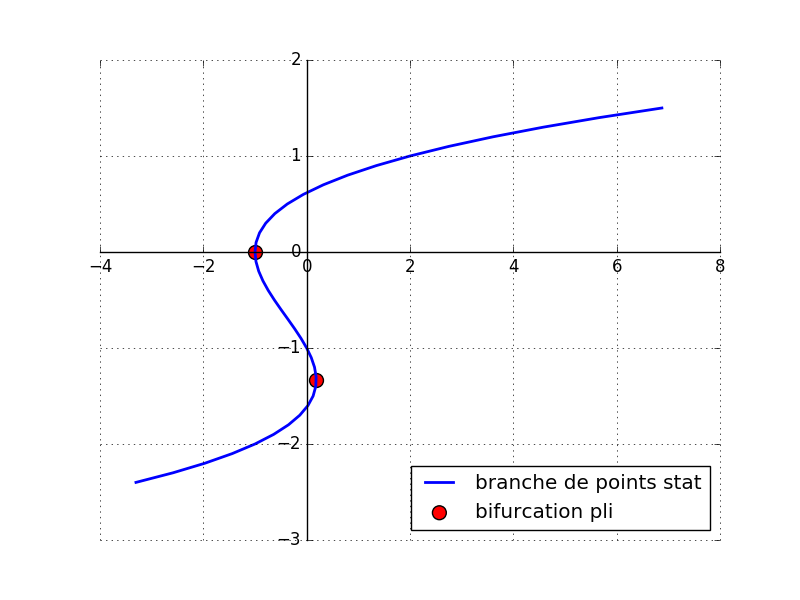
\includegraphics[origin =c, width = 0.7\textwidth]{bifpli.png}
\end{center}
\caption{Bifurcation pli sur le diagramme de bifurcation $v_0=f(I_{ap})$}
\end{figure}
Pour une bifurcation pli, on a l'apparition d'un point stationnaire au point de bifurcation, puis de deux points stationnaires de stabilité oppposé dont un col. Cependant, on a toujours au moins un point stationnaire. La question revient alors à savoir si les branches de points stationnaires nouvelles apparaissent (branches \ref{Branche1}, \ref{Branche2}, \ref{Branche3}) dans la continuité ou non de la branche actuelle (quand $\Delta < 0$, branche \ref{BrancheSolo}). Une condition suffisante pour déterminer, en $I_{ap} = -1$ ou $\frac{5}{27}$, l'emplacement des nouvelles branches apparaissantes par rapport à l'ancienne est comparer leur limite . Si deux nouvelles branches apparaissent sans être dans la continuité de la branche \ref{BrancheSolo}, alors il y a bifurcation pli.

%\textcolor{red}{lim de chaque branche, a la place des sommes d'indicatrice}

\begin{itemize}
\item en $I_{ap} = -1$ à droite de la branche stationnaire \ref{BrancheSolo} avec $\Delta_1 < 0$ et à gauche avec des nouvelles branches stationnaires \ref{Branche1}, \ref{Branche2}, \ref{Branche3} avec $\Delta_1 > 0$
$$\displaystyle{\sum_{i = \ref{Branche1}}^{\ref{Branche3}}\mathds{1}_{\lim\limits_{\substack{I_{ap} \rightarrow -1 \\ I_{ap} < -1}}v_{1, \ref{BrancheSolo}}(I_{ap}), \lim\limits_{\substack{I_{ap} \rightarrow -1 \\ I_{ap} > -1}}v_{1, i}(I_{ap})}} = 1$$
\item en $I_{ap} = \frac{5}{27}$ à droite des branches stationnaires \ref{Branche1}, \ref{Branche2}, \ref{Branche3} avec $\Delta_1 > 0$ et à gauche de l'unique branche \ref{BrancheSolo} avec $\Delta_1 < 0$

$$\displaystyle{\sum_{i = \ref{Branche1}}^{\ref{Branche3}}\mathds{1}_{\lim\limits_{\substack{I_{ap} \rightarrow \frac{5}{27} \\ I_{ap} < \frac{5}{27}}}v_{1, i}(I_{ap}), \lim\limits_{\substack{I_{ap} \rightarrow \frac{5}{27} \\ I_{ap} > \frac{5}{27}}}v_{1, \ref{BrancheSolo}}(I_{ap})}} = 1$$
\end{itemize}

\paragraph{Interprétation avec le diagramme de bifurcation \texorpdfstring{$I_{ap}= f(v_0)$}{Lg}}

\begin{figure}[H]
\begin{center}
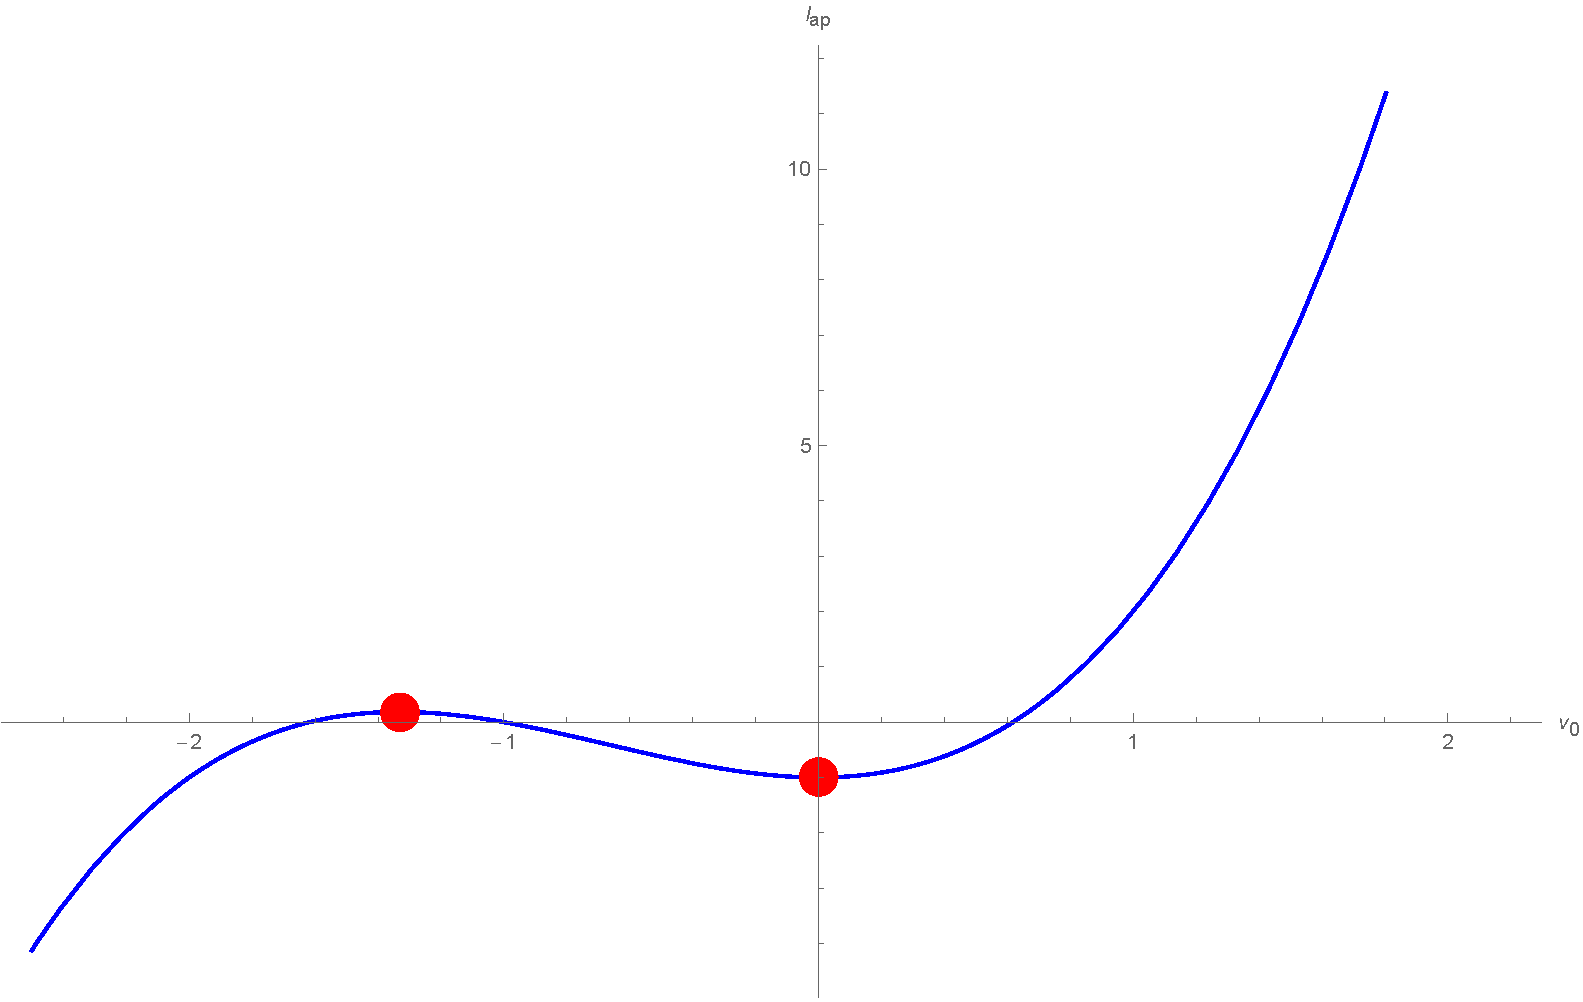
\includegraphics[origin =c, width = 0.8\textwidth]{BifurcationInv}
\end{center}
\caption{Bifurcation pli sur le diagramme de bifurcation $I_{ap}= f(v_0)$}
\end{figure}
Les branches de points stationnaires restent les mêmes que l'on représente $v_0=f(I_{ap})$ ou $I_{ap}= f(v_0)$. Dans cette dernière représentation, les points de bifurcation pli correspondent à des extrema locaux de la fonction $f$ : $v \longmapsto v_0^3 + 2v_0^2 -1 = I_{ap}$.

\begin{align*}
\frac{df}{dv_0} &= 0 \tag*{Extremum local} \\
3v_0^2 + 4v_0 &= 0\\
v_0(3v_0 + 4) &= 0
\end{align*}

Les extrema locaux, et donc les points de bifurcation pli, correspondent à des valeurs de $v_0 = 0$ et $v_0 = -\frac{4}{3}$. Ces valeurs correspondent aux racines (équation \ref{DetJ}) du déterminant de la jacobienne du système. Pour ces valeurs de $v_0$, l'une des deux valeurs propre s'annule. Ainsi, la condition algébrique pour avoir une bifurcation pli sur les valeurs propres de la jacobienne du système est la suivante :

\begin{align}
\text{Bifurcation pli} &\Leftrightarrow \text{Une des valeurs propres de la jacobienne s'annule} \nonumber\\
&\Leftrightarrow v_0 = 0 \quad \text{ou}\quad v_0 = -\frac{4}{3} \label{Bifpli}
\end{align}


\subsubsection{Condition algébrique pour une bifurcation de Hopf}

Pour avoir une bifurcation de Hopf, il faut nécessairement un point stationnaire qui soit un foyer. Pour avoir un foyer en un point $v_0$, il faut que $\Delta < 0$, c'est-à-dire que l'inéquation \ref{DeltaNeg} doit être respectée. De plus, une bifurcation de Hopf ne peut avoir lieu que lors de la transition d'un foyer stable à un foyer instable. Les conditions algébriques pour une bifurcation de Hopf en un point $v_H$ sont les suivantes :
\begin{equation}
	\left\{
		\begin{array}{ll}
			v < v_H & \text{foyer stable ou instable}\\
			v > v_H & \text{foyer de stabilité opposée}\\
			\left.\dfrac{dRe(\lambda)}{dI_{ap}}\right|_{v_H} \ne 0 &  \Leftrightarrow \left.\dfrac{d\left(\frac{3v_0}{2c}((2-v_0) - 1)\right)}{dI_{ap}}\right|_{v_H} \ne 0\\
		\end{array}
	\right.
\label{BifHopf}
\end{equation}

\subsubsection{Résumé des stabilités et des bifurcations}

D'après les équations \ref{TrJ} et \ref{DetJ}, et à l'aide du théorème de Hartman-Grobam, on peut déduire la nature des points d'équilibre dans les deux tableaux \ref{resume_c_1} et \ref{resume_c_2}.
A l'aide des conditions de bifurcation pli \ref{Bifpli} et de Hopf \ref{BifHopf}, validées pour certaines valeurs de $v_0$, on a alors le résumé suivant pour $c=1$ et $c=2$.

Ces résultats théoriques ont été validés à l'aide de \texttt{XPP-aut}, dont les diagrammes de bifurcation obtenus par continuation sont présentés en figure \ref{fig_res_c_2} et \ref{fig_res_c_1}

\newpage

\begin{table}[H]
\begin{tabular}{|L{2cm} | C{2cm} | C{2.5cm} | C{2.5cm} |C{2.5cm}|C{2.5cm}|}
\hline
\multicolumn{6}{|c|}{$c = 2$}
\\\hline
Valeur de $v_0$ & $v_0 < - \frac{4}{3}$ & $- \frac{4}{3} < v_0 < 0$ & $0 < v_0 < 1 - \frac{\sqrt{3}}{3}$ & $1 - \frac{\sqrt{3}}{3} < v_0 < 1 + \frac{\sqrt{3}}{3}$ &$v_0 > 1 + \frac{\sqrt{3}}{3}$ \\
 \hline
$Tr(J)$ & - & - & - & + & - \\ \hline
$Det(J)$ & + & - & + & + &+ \\ \hline
Nature & foyer ou noeud stable  & col & foyer ou noeud stable & foyer ou noeud instable & foyer ou noeud stable \\ \hline
\end{tabular}
\caption{Résumé de la stabilité des points d'équilibre pour $c = 2$}
\label{resume_c_1}
\end{table}

\begin{figure}[H]
\begin{center}
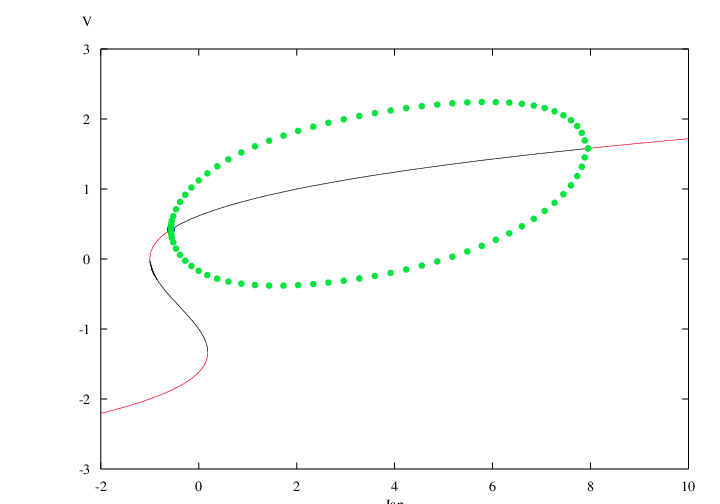
\includegraphics[width = 1.0\textwidth]{bif_20.png}
\end{center}
\caption{Diagramme de bifurcation $v_0=f(I_{ap})$ obtenu pour $c=2$ à l'aide de \texttt{XPP-aut} par continuation. Les familles de points stationnaires stables sont représentées en trait continu rouge, les familles de points stationnaires instables en trait continu noir, et les familles de cycles limites stables en pointillés vert}
\label{fig_res_c_2}
\end{figure}


\textbf{Pour $c=2$}, il y a deux bifurcations de Hopf en $v_0 = 1 - \frac{\sqrt{3}}{3}$ et en $v_0 = 1 + \frac{\sqrt{3}}{3}$. Il y a également deux bifurcation pli en $v_0 = 0$ et $v_0 = -\frac{4}{3}$.

\newpage

\begin{table}[H]
\begin{tabular}{|L{2cm} | C{2cm} | C{2.5cm} | C{2.5cm} |C{2.5cm}|C{2.5cm}|}
\hline
\multicolumn{6}{|c|}{$c = 1$}
\\\hline
Valeur de $v_0$ & $v_0 < - \frac{4}{3}$ & $- \frac{4}{3} < v_0 < 0$ & $0 < v_0 < 1 - \sqrt{\frac{2}{3}}$ & $1 - \sqrt{\frac{2}{3}} < v_0 < 1 + \sqrt{\frac{2}{3}}$ &$v_0 > 1 + \sqrt{\frac{2}{3}}$ \\
 \hline
$Tr(J)$ & - & - & - & + & - \\ \hline
$Det(J)$ & + & - & + & + &+ \\ \hline
Nature & foyer ou noeud stable  & col & foyer ou noeud stable & foyer ou noeud instable & foyer ou noeud stable \\ \hline
\end{tabular}
\caption{Résumé de la stabilité des points d'équilibre pour $c = 1$}
\label{resume_c_2}
\end{table}

\begin{figure}[H]
\begin{center}
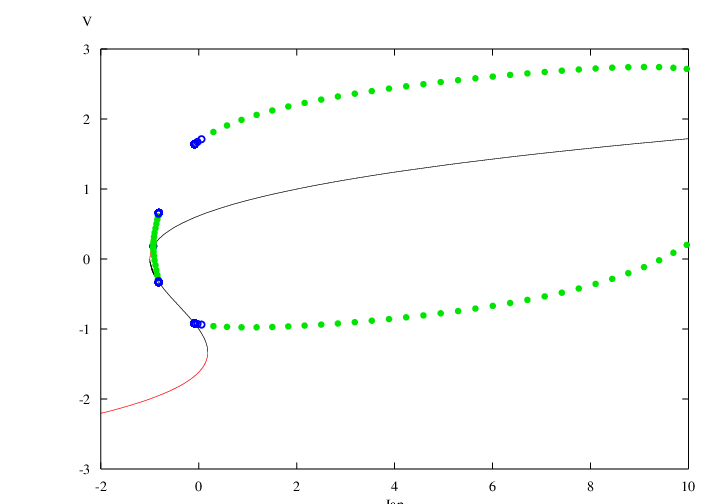
\includegraphics[width = 1.0\textwidth]{bif_10.png}
\end{center}
\caption{Diagramme de bifurcation $v_0=f(I_{ap})$ obtenu pour $c=1$ à l'aide de \texttt{XPP-aut} par continuation. Les familles de points stationnaires stables sont représentées en trait continu rouge, les familles de points stationnaires instables en trait continu noir, et les familles de cycles limites stables en pointillés vert. Les points bleus correspondent aux points pour lesquels la période des solutions attirés par les cylces limites stables tend vers l'infini}
\label{fig_res_c_1}
\end{figure}

\textbf{Pour $c=1$}, il y a deux bifurcations de Hopf en $v_0 = 1 - \sqrt{\frac{2}{3}}$ et en $v_0 = 1 + \sqrt{\frac{2}{3}}$. Il y a également deux bifurcation pli en $v_0 = 0$ et $v_0 = -\frac{4}{3}$.




%On a alors :
%$$x_{Tr+} = 1 + \frac{\sqrt{3}}{3} \quad \text{et}\quad x_{Tr-} = 1 - \frac{\sqrt{3}}{3}$$



\newpage

\section{Simulations numériques}
	\subsection{Pour $c=2$}
		\subsubsection{Simulations pour $I_{ap}$ entre -2 et 10}

Comme nous l'avons précédemment vu le nombre de point stationnaire et leur stabilité dépend de $I_{ap}$. Nous avons réalisé nos simulations à l'aide de \texttt{XPP-aut}, dans lesquelles une variation de $I_{ap}$ permet de parcourir tout le diagramme de bifurcation, comme le montre l'équation \ref{Stat}.



\paragraph{$I_{ap}$ entre -2 et -1}
Il n'y a qu'un point d'équilibre : un noeud stable.

\begin{figure}[H]
\begin{center}
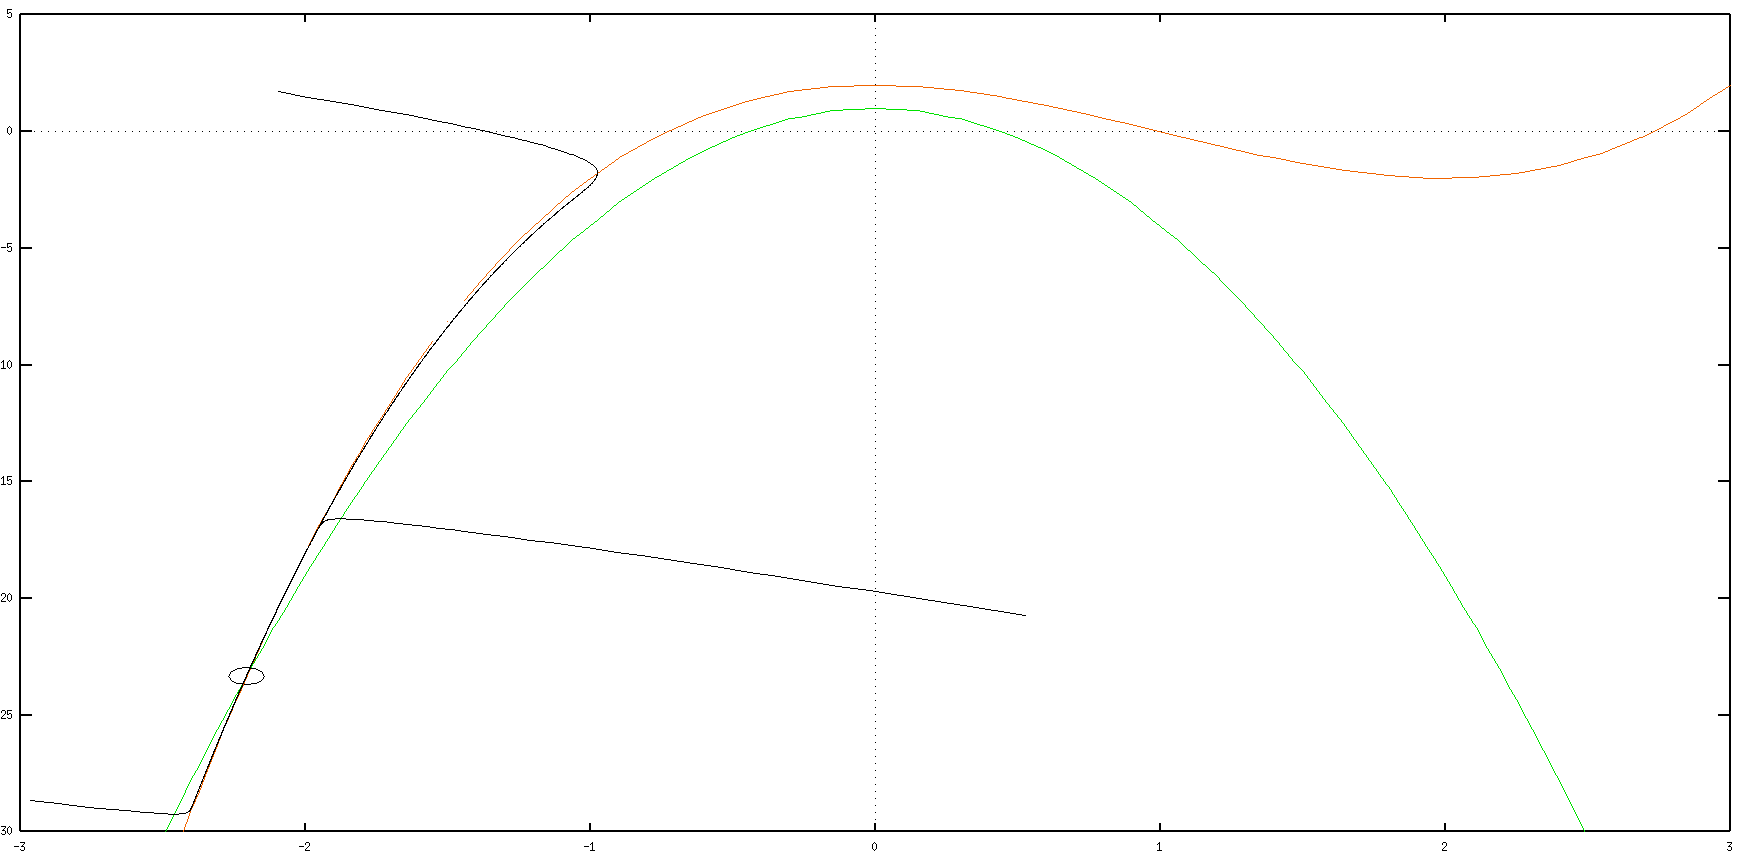
\includegraphics[ width = 0.7\textwidth]{I_000.png}
\end{center}
\caption{Plan de phase pour $I=-2$, le point stationnaire est un noeud stable}
\end{figure}


\paragraph{À $I_{ap}=-1$}
Bifurcation pli, apparition d'un nouveau point d'équilibre.

\begin{figure}[H]
\begin{center}
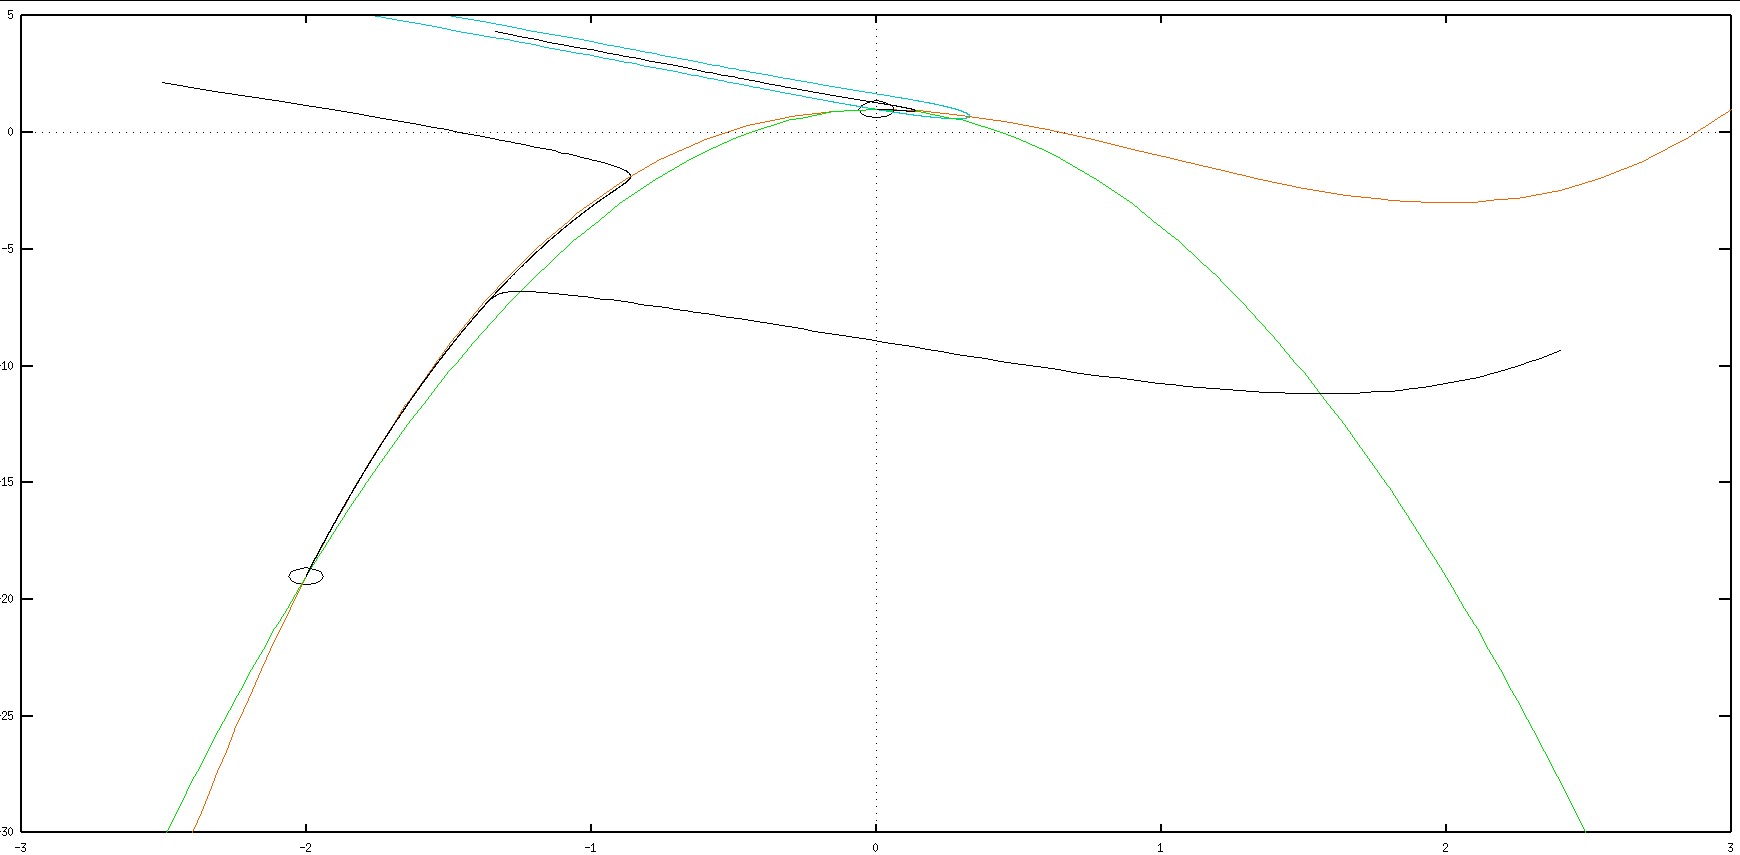
\includegraphics[ width = 0.7\textwidth]{I_003.png}
\end{center}
\caption{Plan de phase $w=f(v)$ pour $I=-1$, deux points stationnaires}
\end{figure}

\paragraph{$I_{ap}$ entre -1 et -0.5672}
3 points stationnaires : un noeud stable, un col et un autre noeud stable qui devient ensuite un foyer stable. La varitété instable du col sépare les deux bassins d'attraction de chaque noeud.

\begin{figure}[H]
\begin{center}
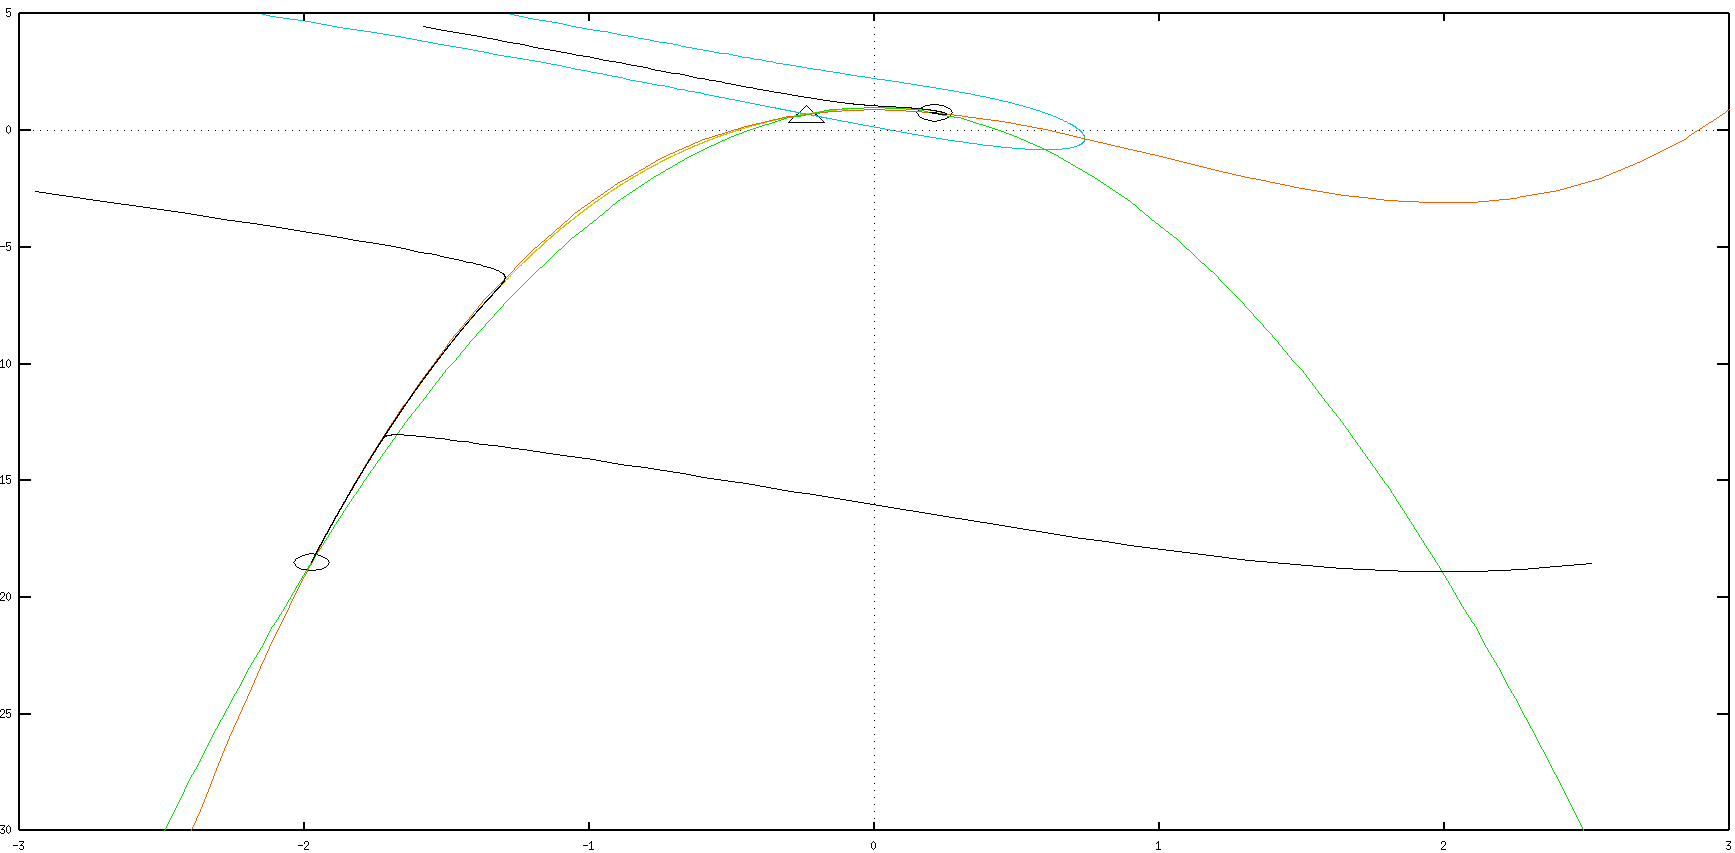
\includegraphics[ width = 0.5\textwidth]{I_004.png}
\end{center}
\caption{Plan de phase $w=f(v)$, trois points stationnaires : 2 stables et 1 col.}
\end{figure}

\paragraph{$I_{ap}$ entre -0.5672 et 0.185}
Bifurcation de Hopf : le foyer stable devient instable et un cycle limite stable apparaît. Quand $I_{ap}$ augmente, le cycle limite stable grossit.
On compte 3 points stationnaires.
\begin{figure}[H]
\begin{center}
\begin{tabular}{ p{0.5\textwidth}  p{0.5\textwidth} }
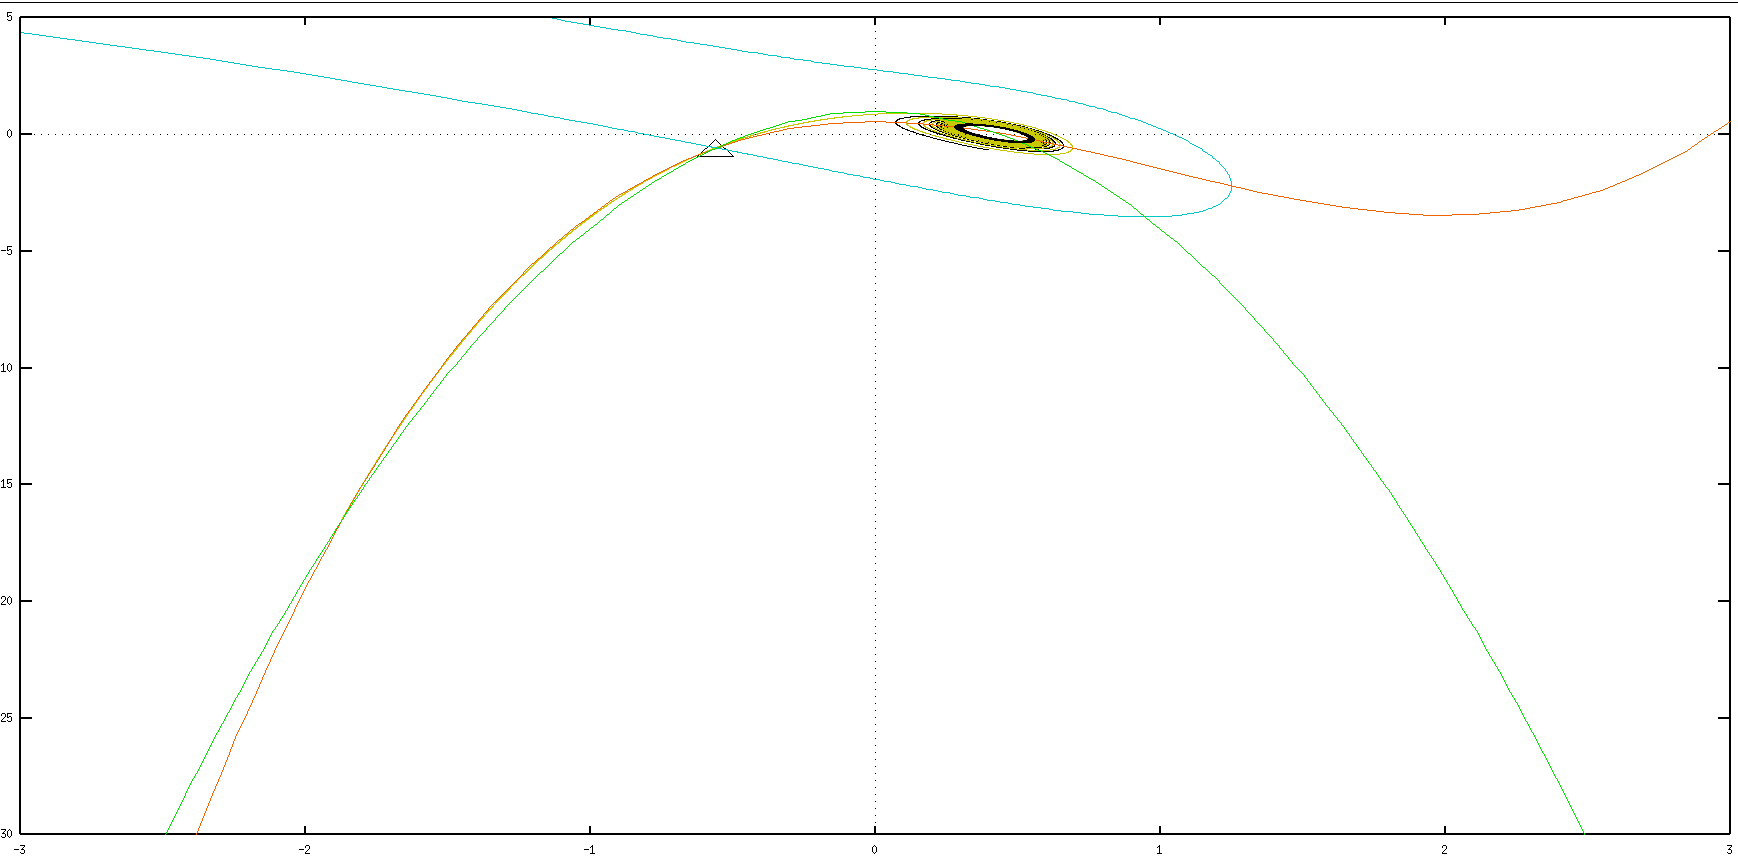
\includegraphics[ width = 0.5\textwidth]{I_007.png} &
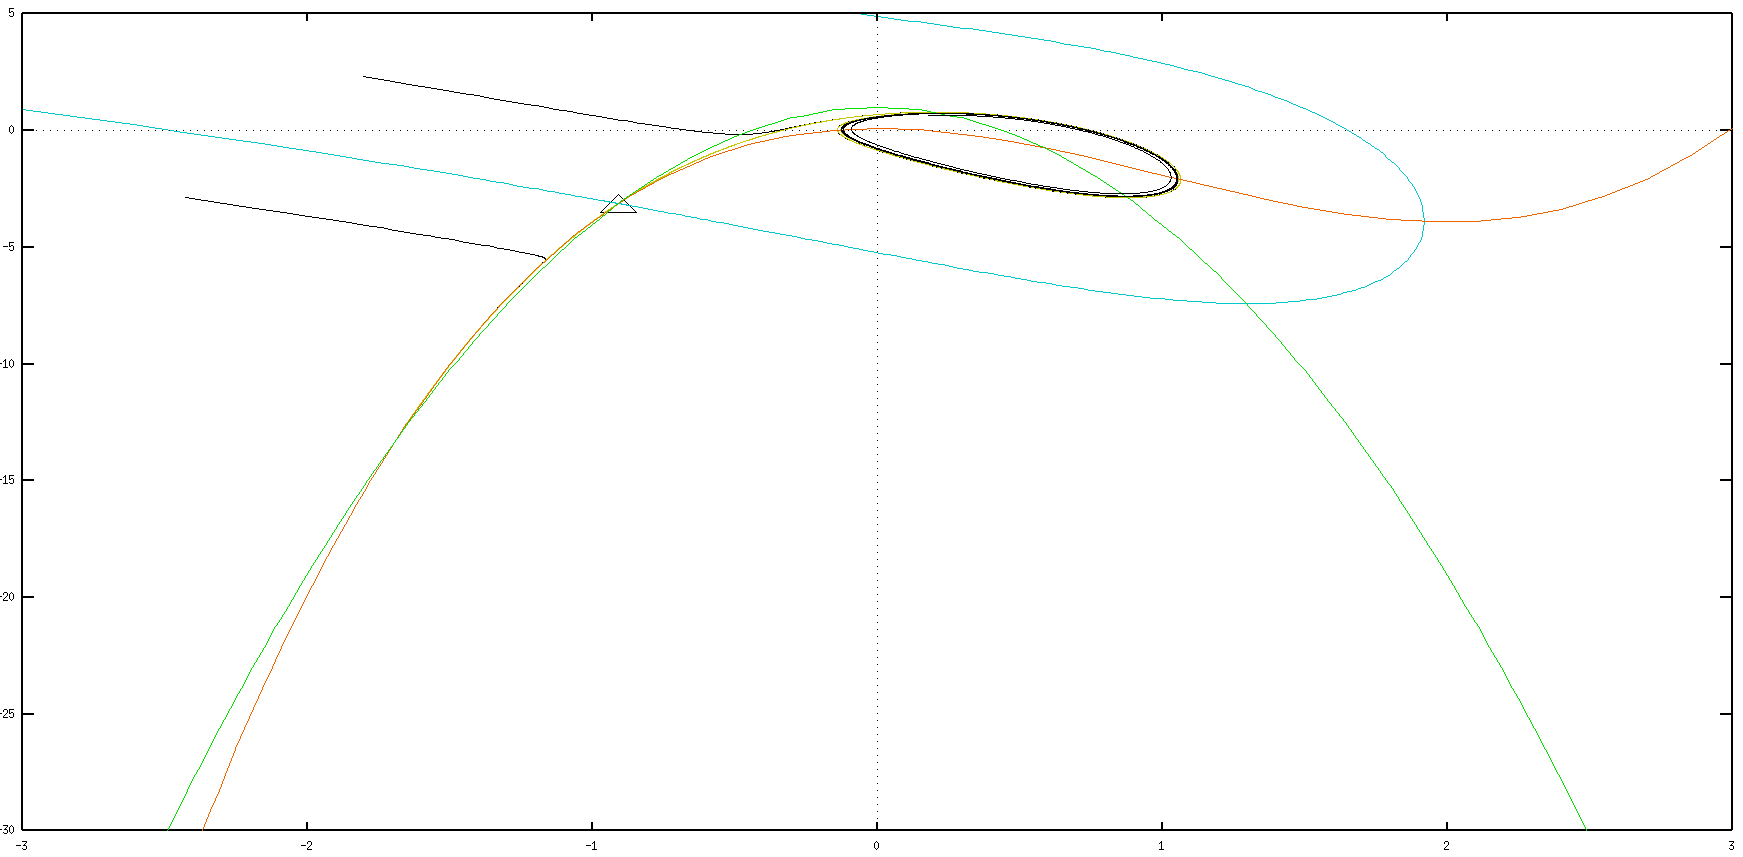
\includegraphics[ width = 0.5\textwidth]{I_008.png}
\end{tabular}
\end{center}
\caption{Plan de phase $w=f(v)$, trois points stationnaires et un cycle limite stable.}
\end{figure}

\paragraph{À $I_{ap} \approx 0.185$}
Bifurcation pli, le col et le noeud stable se rejoingne pour ne former qu'un seul point, puis disparaissent.
\begin{figure}[H]
\begin{center}
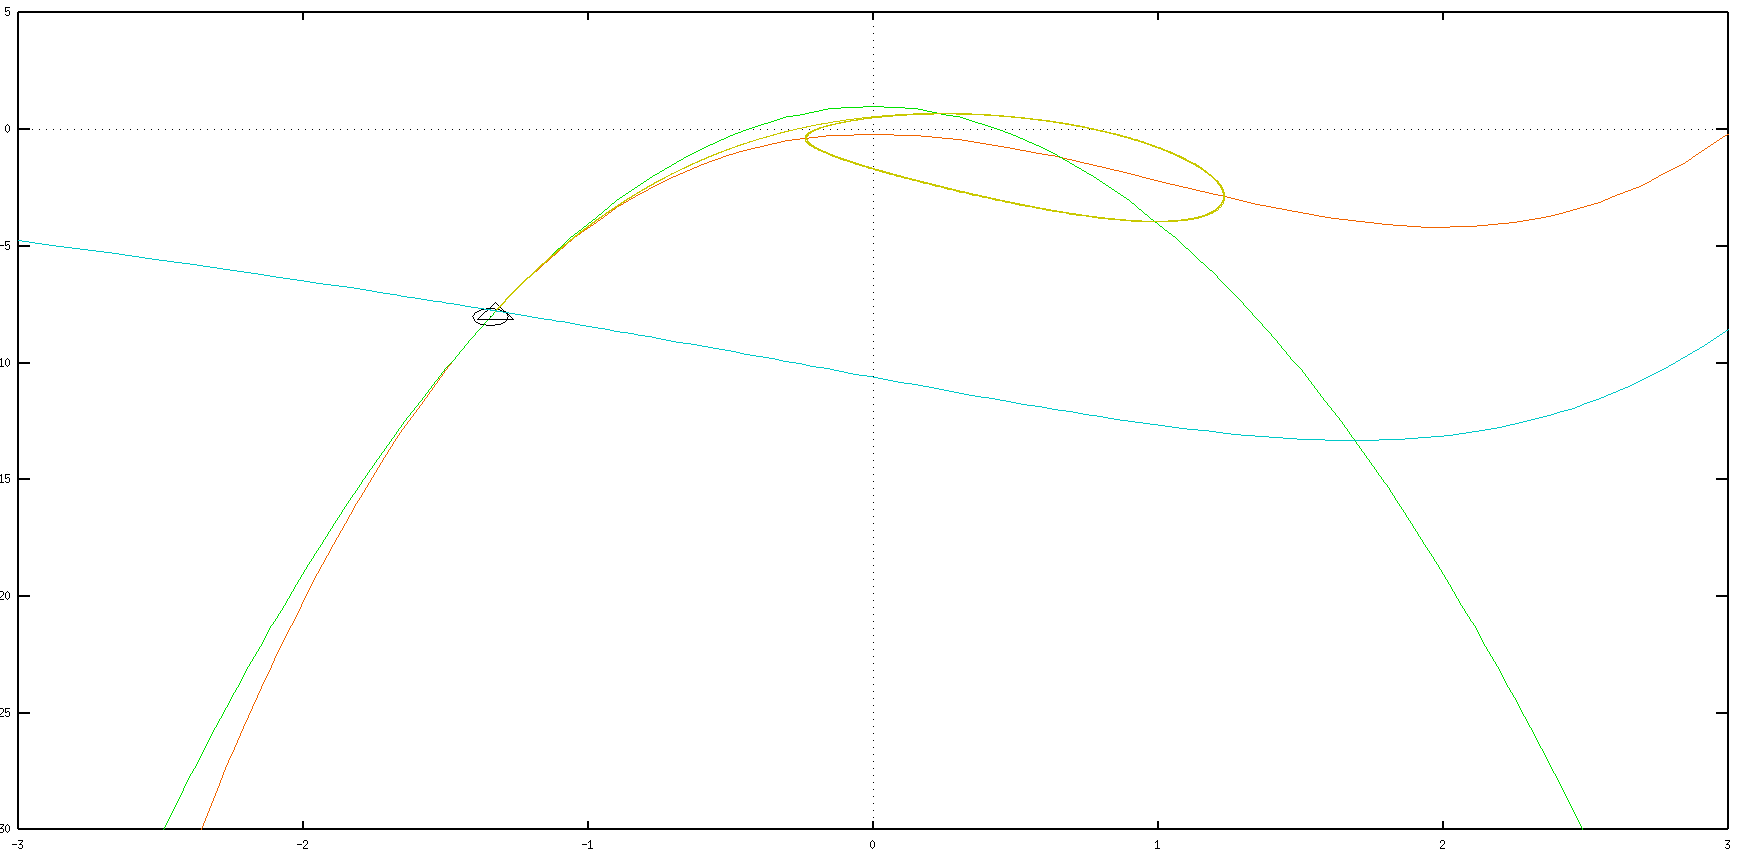
\includegraphics[ width = 0.5\textwidth]{I_011.png}
\end{center}
\caption{Plan de phase $w=f(v)$, deux points stationnaires et un cycle limite stable.}
\end{figure}

\paragraph{$I_{ap}$ entre 0.185 et 7.9}
Il n'y a plus qu'un point stationnaire : le foyer instable. Le cycle limite grossit puis diminue.
\begin{figure}[H]
\begin{center}
\begin{tabular}{ p{0.5\textwidth}  p{0.5\textwidth} }
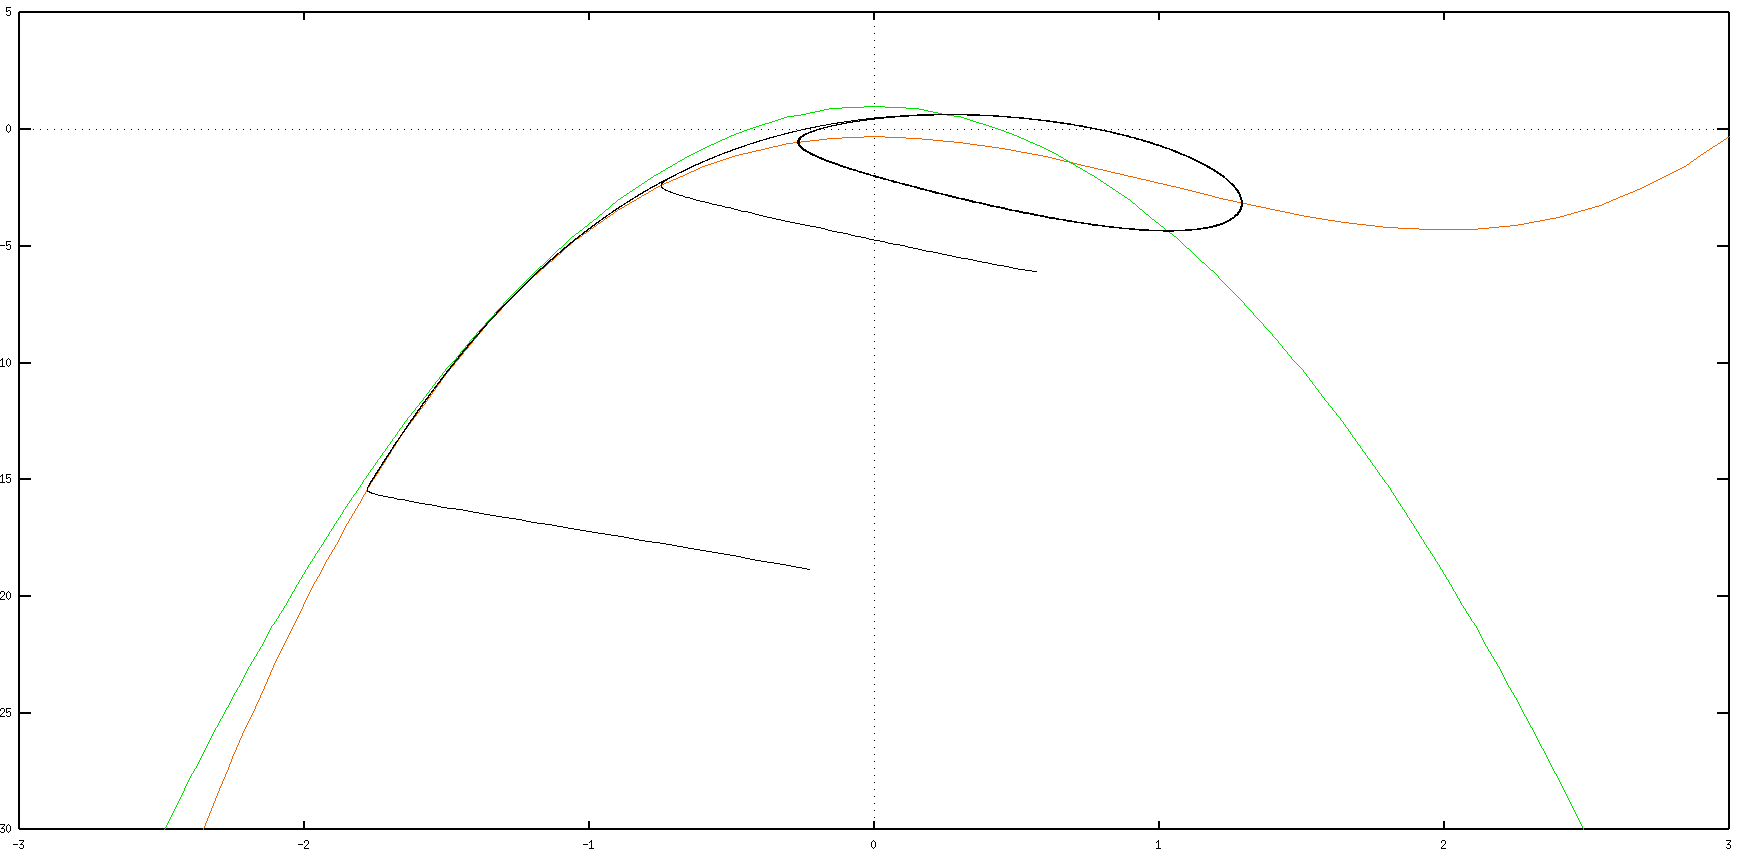
\includegraphics[ width = 0.5\textwidth]{I_012.png} &
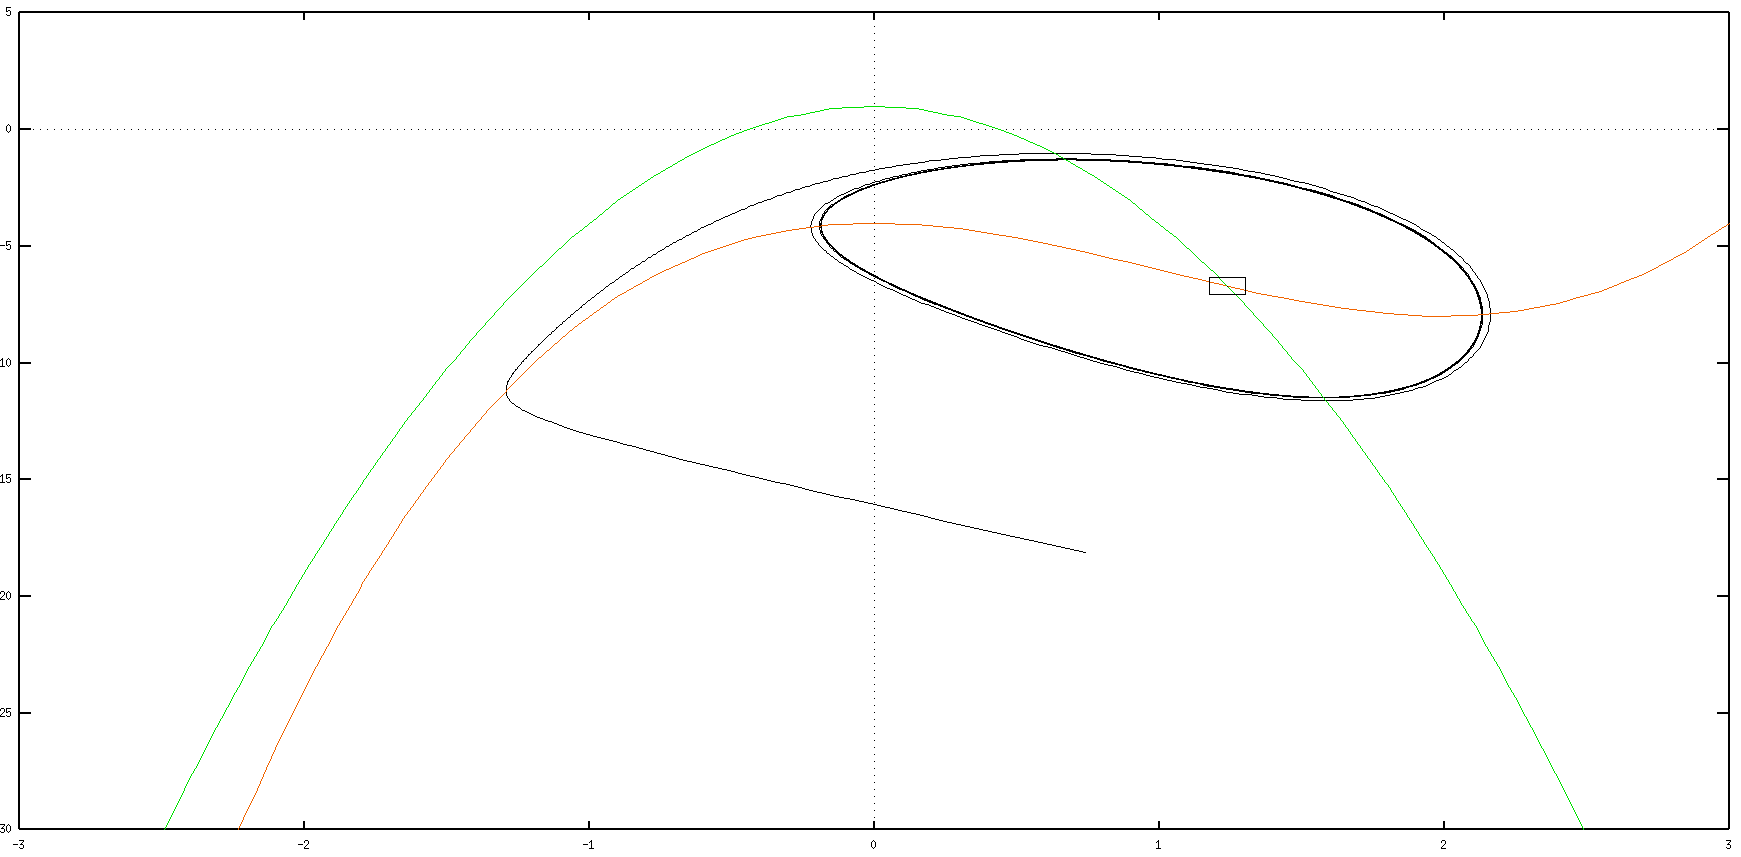
\includegraphics[ width = 0.5\textwidth]{I_013.png} \\
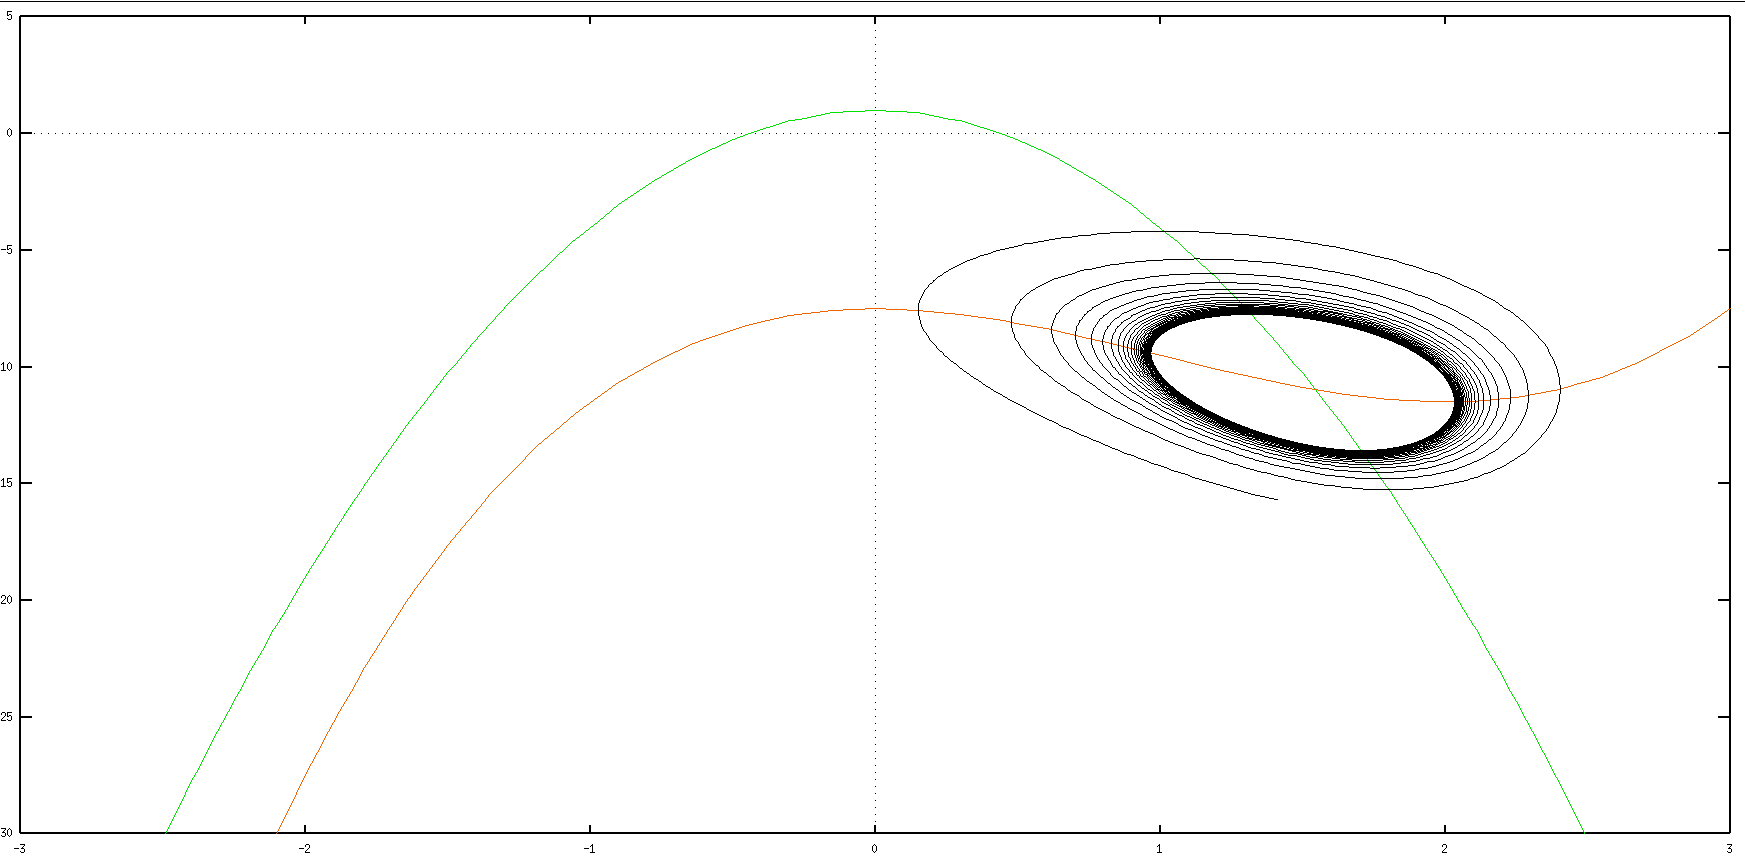
\includegraphics[ width = 0.5\textwidth]{I_015.png} &
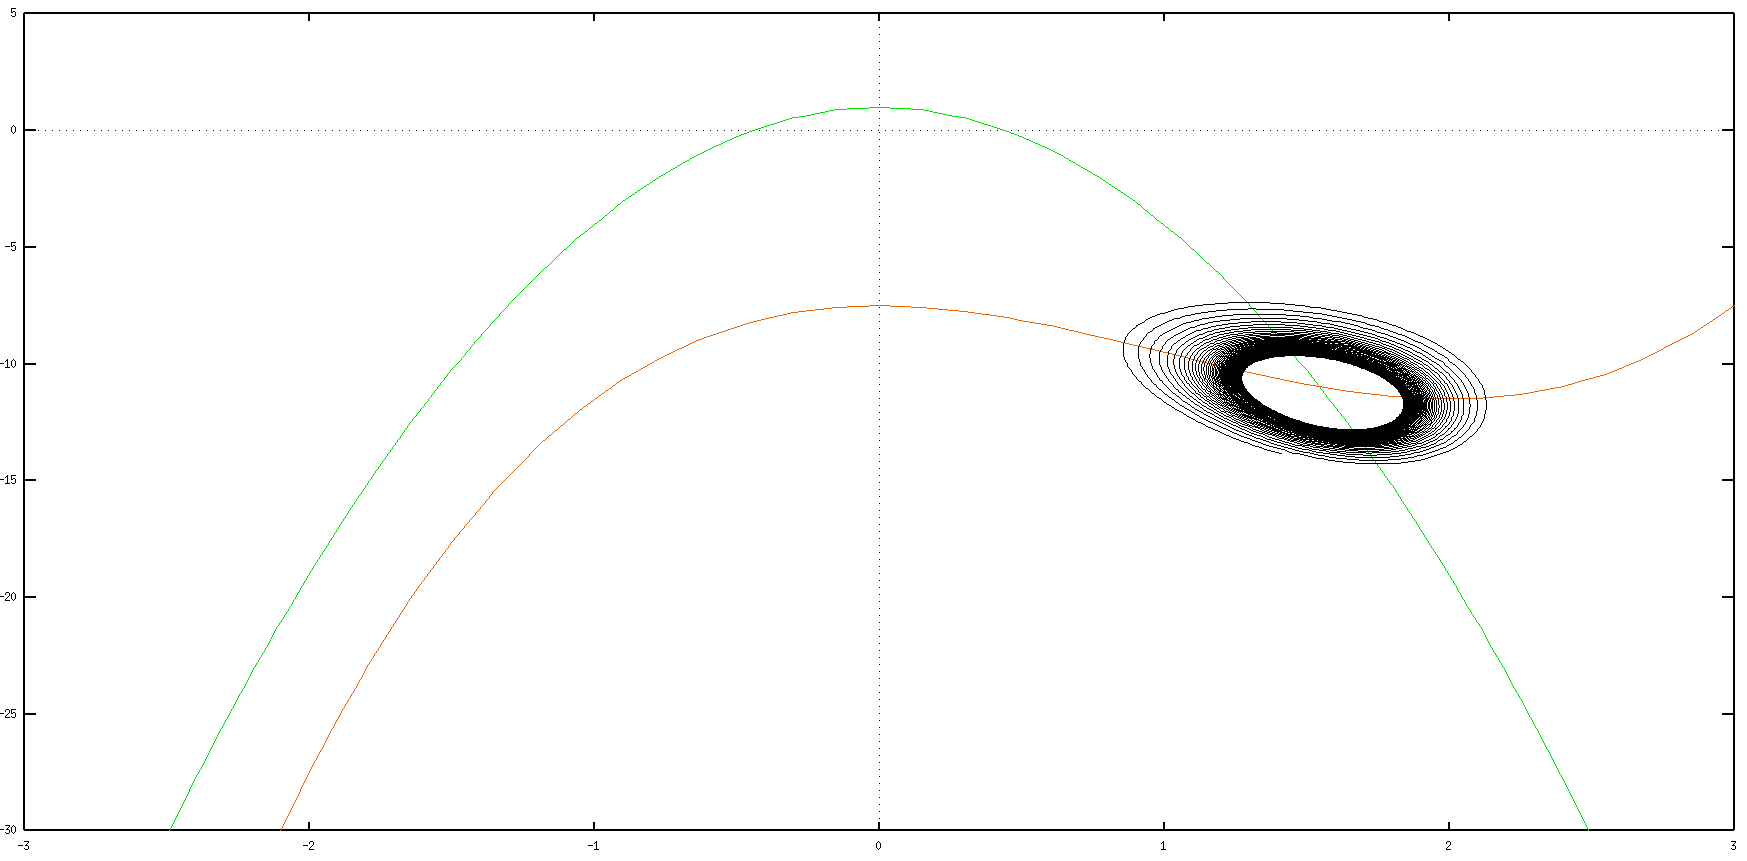
\includegraphics[ width = 0.5\textwidth]{I_016.png} \\
\end{tabular}
\end{center}
\caption{Plan de phase $w=f(v)$, un foyer instable et un cycle limite stable dont la taille augmente puis diminue.}
\end{figure}

\paragraph{$I_{ap}$ entre $7.9001$ et $10$}
Bifurcation de Hopf, le cycle limite stable disparaît. Le foyer instable devient un foyer stable.
\begin{figure}[H]
\begin{center}
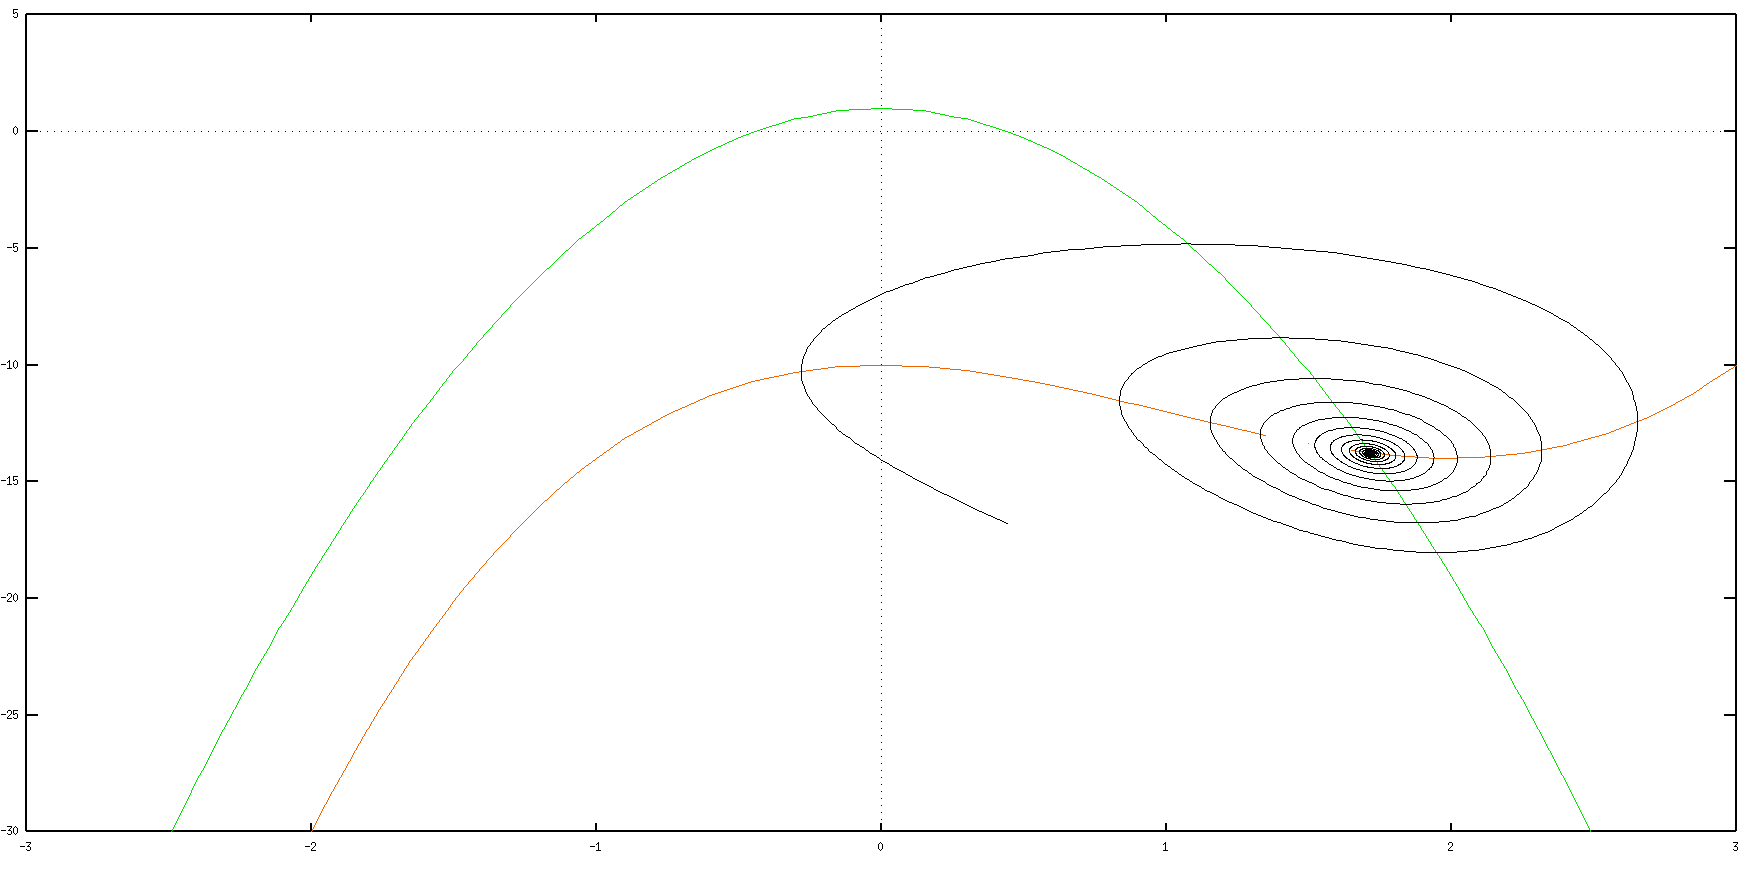
\includegraphics[ width = 0.7\textwidth]{I_018.png}
\end{center}
\caption{Plan de phase $w=f(v)$, un foyer stable.}
\end{figure}

\newpage


\subsubsection{Résumé pour $c=2$}


\begin{tabular}{|C{4.5cm} | C{2.2cm} | C{8cm}  |}
\hline
\rowcolor{maroon}
Valeur de $I_{ap}$ & Nombre de points stat & Caractérisation des points \\
\rowcolor{maroon!10}
$I_{ap} \in [-2, -1[$ & 1 & noeud stable \\
\rowcolor{maroon!50}
$I_{ap} = -1$ & 2 & \textcolor{white}{\textbf{Bifurcation pli}} \newline noeud stable et \textbf{col-noeud} \\
\rowcolor{maroon!10}
$I_{ap} \in [-1, -0.9880[$ & 3 & noeud stable et \textbf{col} et \textbf{noeud stable} \\\hline
\rowcolor{maroon!10}
$I_{ap} \in [-0.9880, -0.5672[$ & 3 & noeud stable et col et \textbf{foyer stable} \\
\rowcolor{maroon!50}
$I_{ap} \approx -0.5672$ &
\multicolumn{2}{c|}{\textcolor{white}{\textbf{Bifurcation Hopf}}} \\
\rowcolor{maroon!10}
$I_{ap} \in ]-0.5672, 5/27[$ & 3 & noeud stable et col et \textbf{foyer instable et cycle limite stable} \\\hline
\rowcolor{maroon!50}
$I_{ap} = 5/27$ & 2 & \textcolor{white}{\textbf{Bifurcation pli}} \newline foyer instable, cycle limite stable et \textbf{col-noeud} \\
\rowcolor{maroon!10}
$I_{ap} \in ]5/27, 7.9001[$ & 1 &  foyer instable et cycle limite stable\\
\rowcolor{maroon!50}
$I_{ap} \approx 7.9001$ &
\multicolumn{2}{c|}{\textcolor{white}{\textbf{Bifurcation Hopf}}} \\
\rowcolor{maroon!10}
$I_{ap} \in ]7.9001, 10[$ & 1 &   foyer stable \\\hline
\end{tabular}
\vspace*{0,3cm}


\begin{figure}[H]
\begin{center}
	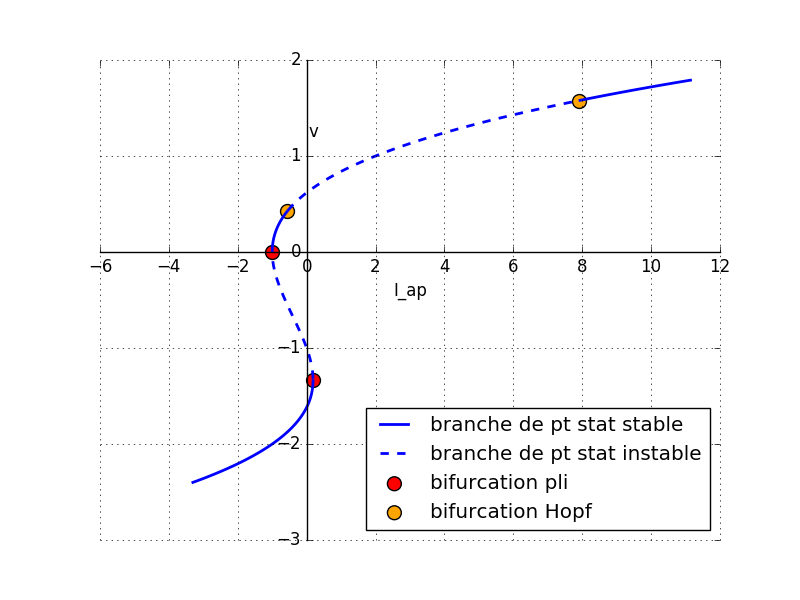
\includegraphics[ width = 0.8\textwidth]{bif4.png}
\end{center}
\caption{A gauche : diagramme de bifurcation théorique (la famille de cycle limite n'est pas représentée). Le diagramme de bifurcation obtenu par continuation avec \texttt{XXP-aut} a déjà été présenté en figure \ref{fig_res_c_2}}
\end{figure}


\vspace*{0,3cm}

Le système possède des régions de \textbf{bistabilité} :
\begin{itemize}
\item Pour $I_{ap} \in ]-1, -0,5672[$ : deux famille de points stationnaires stables co-existent.
\item Pour  $I_{ap} \in ] -0,5672, 5/27[$ une famille de points stationnaires stables co-existe avec une famille de cycle limite stable
\end{itemize}
C'est à dire, il y a bi-stabilité entre les deux bifurcations pli.


\newpage
\subsection{Pour $c=1$}


Les bifurcations plis observées pour $c=2$ restent inchangées mais les bifurcations de Hopf s'éloignent l'une de l'autre (que ce soit par rapport à $v$ ou $I_{ap}$). Contrairement à $c = 2$, il y a deux bifurcations homoclines (pour $I_{ap} = -0.8161$ et $I_{ap} = -0.08560$), faisant disparaître puis réapparaître le cycle limite stable.

\subsubsection{Simulations numériques pour $I_{ap}$ entre $-2$ et $10$}

\paragraph{Pour $I_{ap}$ entre -2 et -1}
On commence avec un noeud stable. La nullcline pour $v$ se rapproche du sommet de la nullcline de $w$ quand $I_{ap}$ augmente.
\begin{figure}[H]
	\begin{center}
	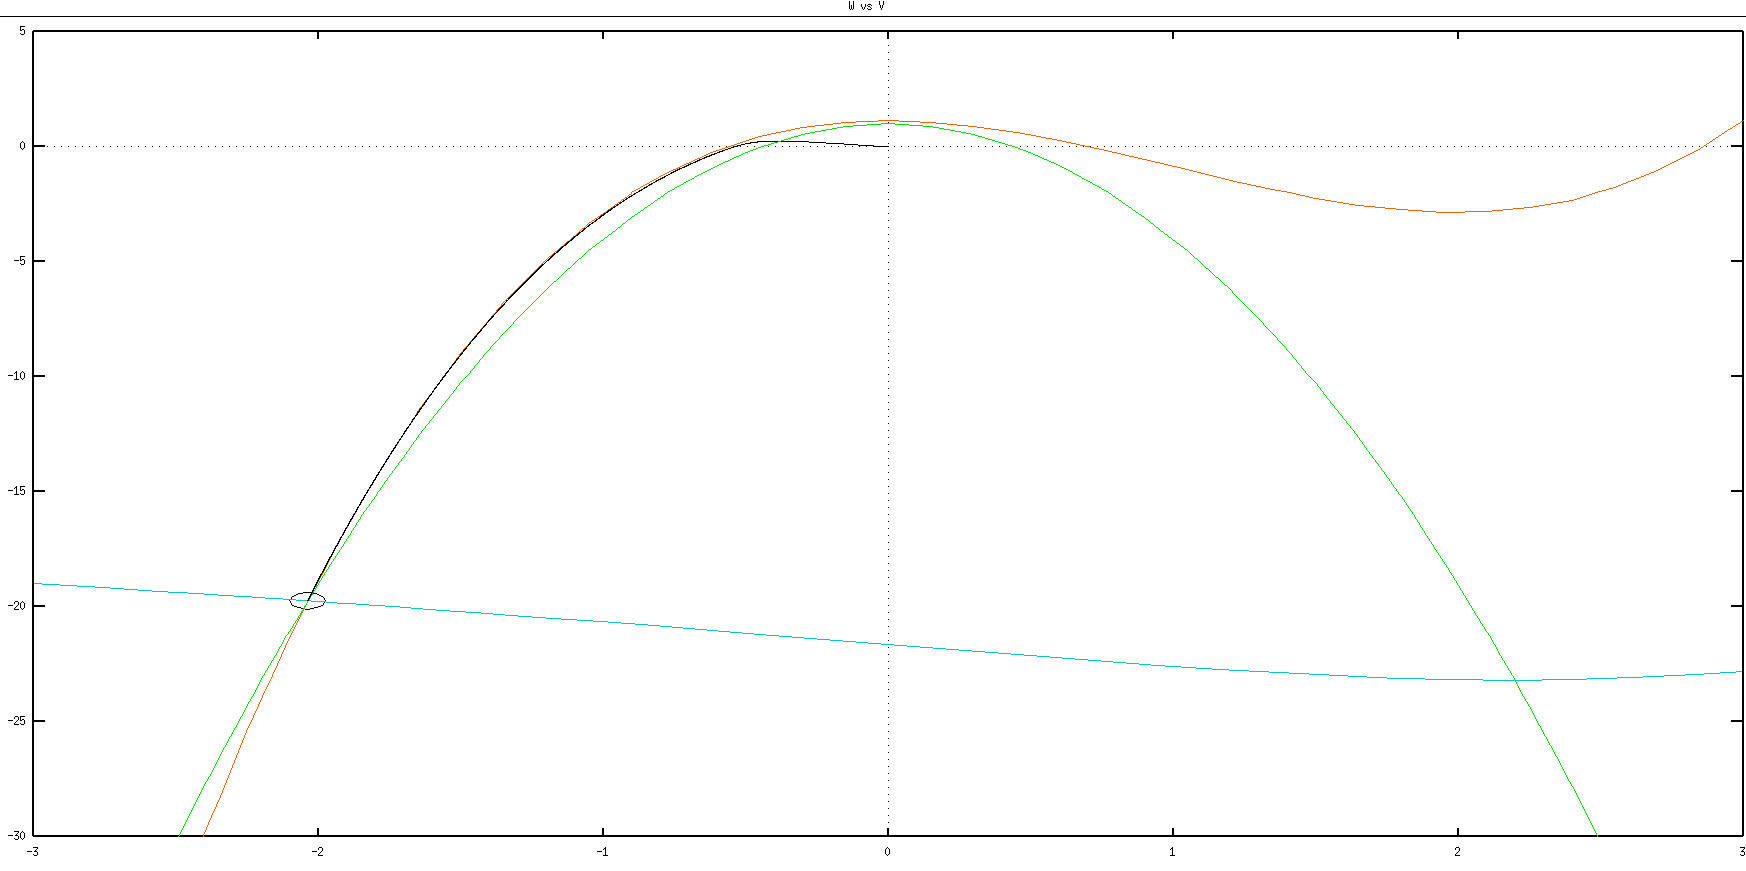
\includegraphics[ width = 0.7\textwidth]{3I-1_15.png}
	\end{center}
\caption{Plan de phase $w=f(v)$ pour $I_{ap} = -1.15$ : 1 noeud stable}
\end{figure}

\paragraph{À $I_{ap}=-1$}
Pour cette valeur de $I_{ap}$ les deux nullclines coïncident au point du sommet de la nullcline pour $w$, et on a apparition d'un col noeud : c'est la première bifurcation pli.
\begin{figure}[H]
	\begin{center}
	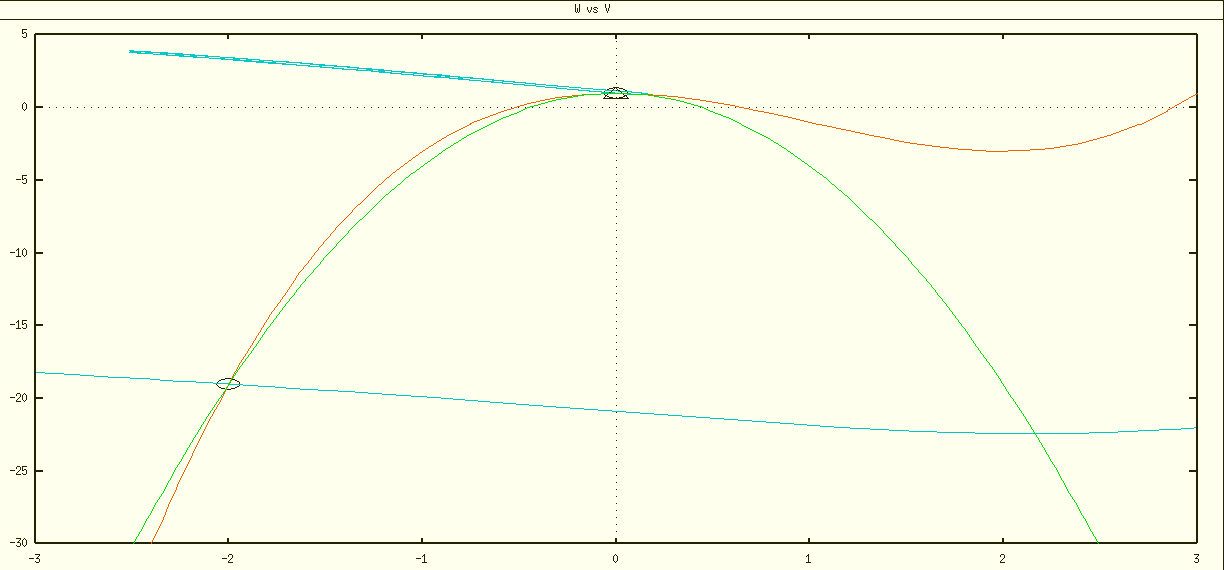
\includegraphics[ width = 0.7\textwidth]{I-1.png}
	\end{center}
\caption{Plan de phase $w=f(v)$ pour $I_{ap} = -1$ : 1 noeud stable et apparition d'un col-noeud}
\end{figure}


\paragraph{Pour $I_{ap}$ entre -1 et -0.9265}
Après la bifurcation pli, il y a 2 attracteurs, 1 noeud stable, et un autre noeud stable isssu de la bifurcation pli qui devient foyer stable. Les bassins d'attraction de ces deux attracteurs sont séparés par la variété instable du col.
\begin{figure}[H]
\begin{center}
\begin{tabular}{p{0.5\textwidth}  p{0.5\textwidth}}
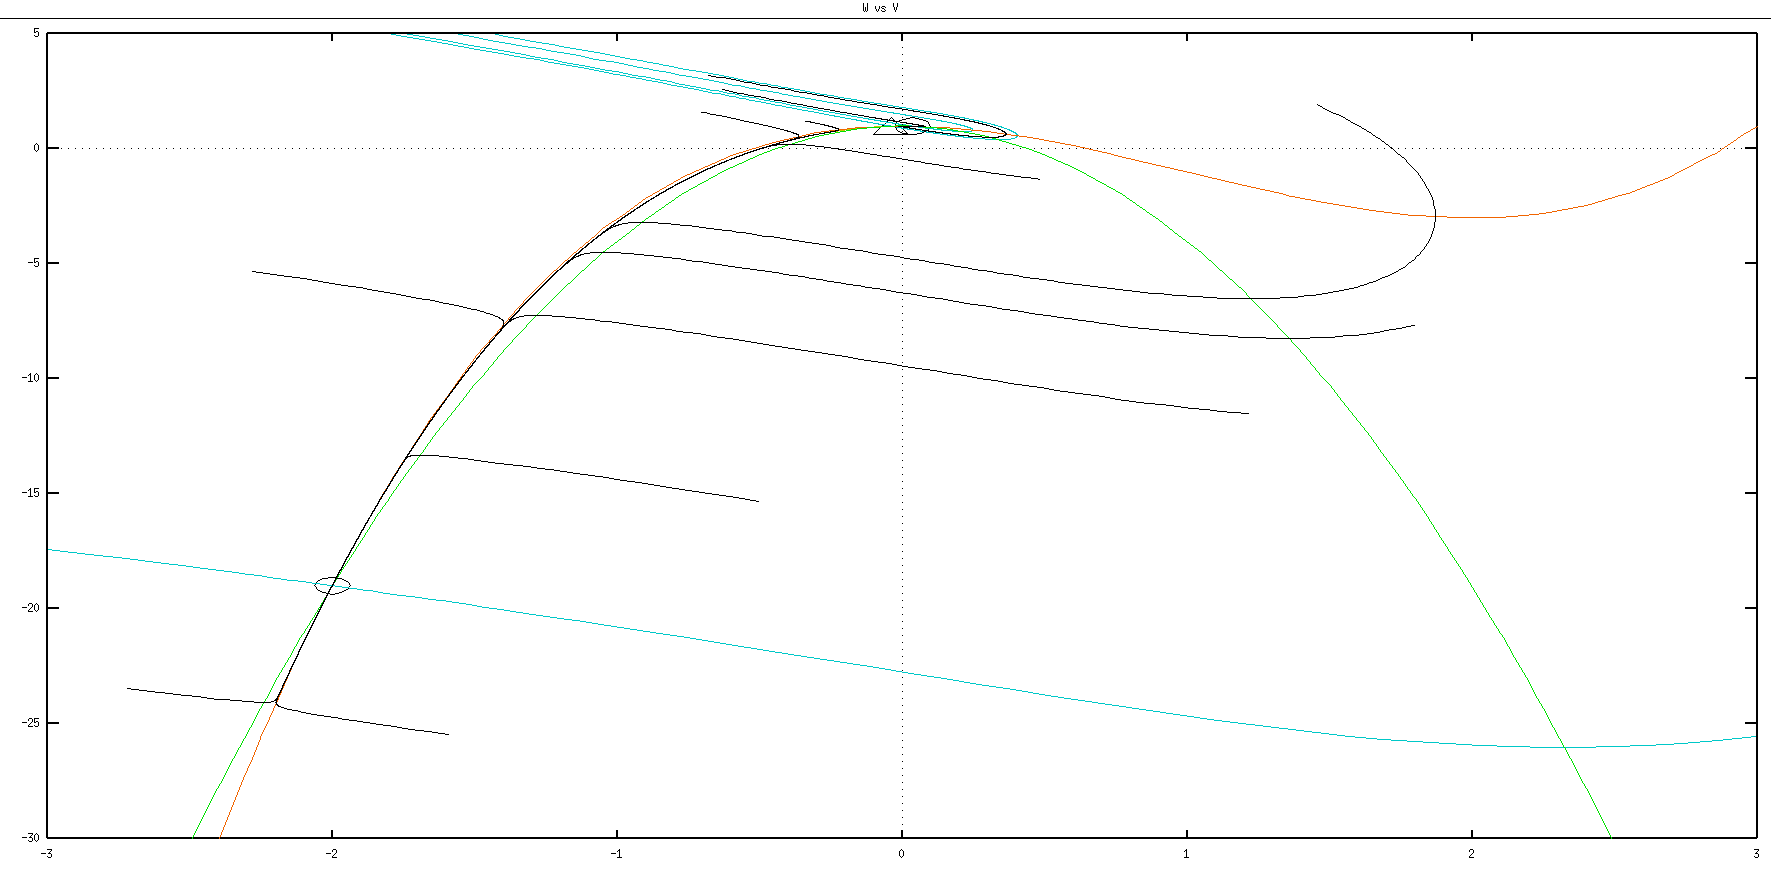
\includegraphics[ width = 0.5\textwidth]{6I-0_9971.png} &
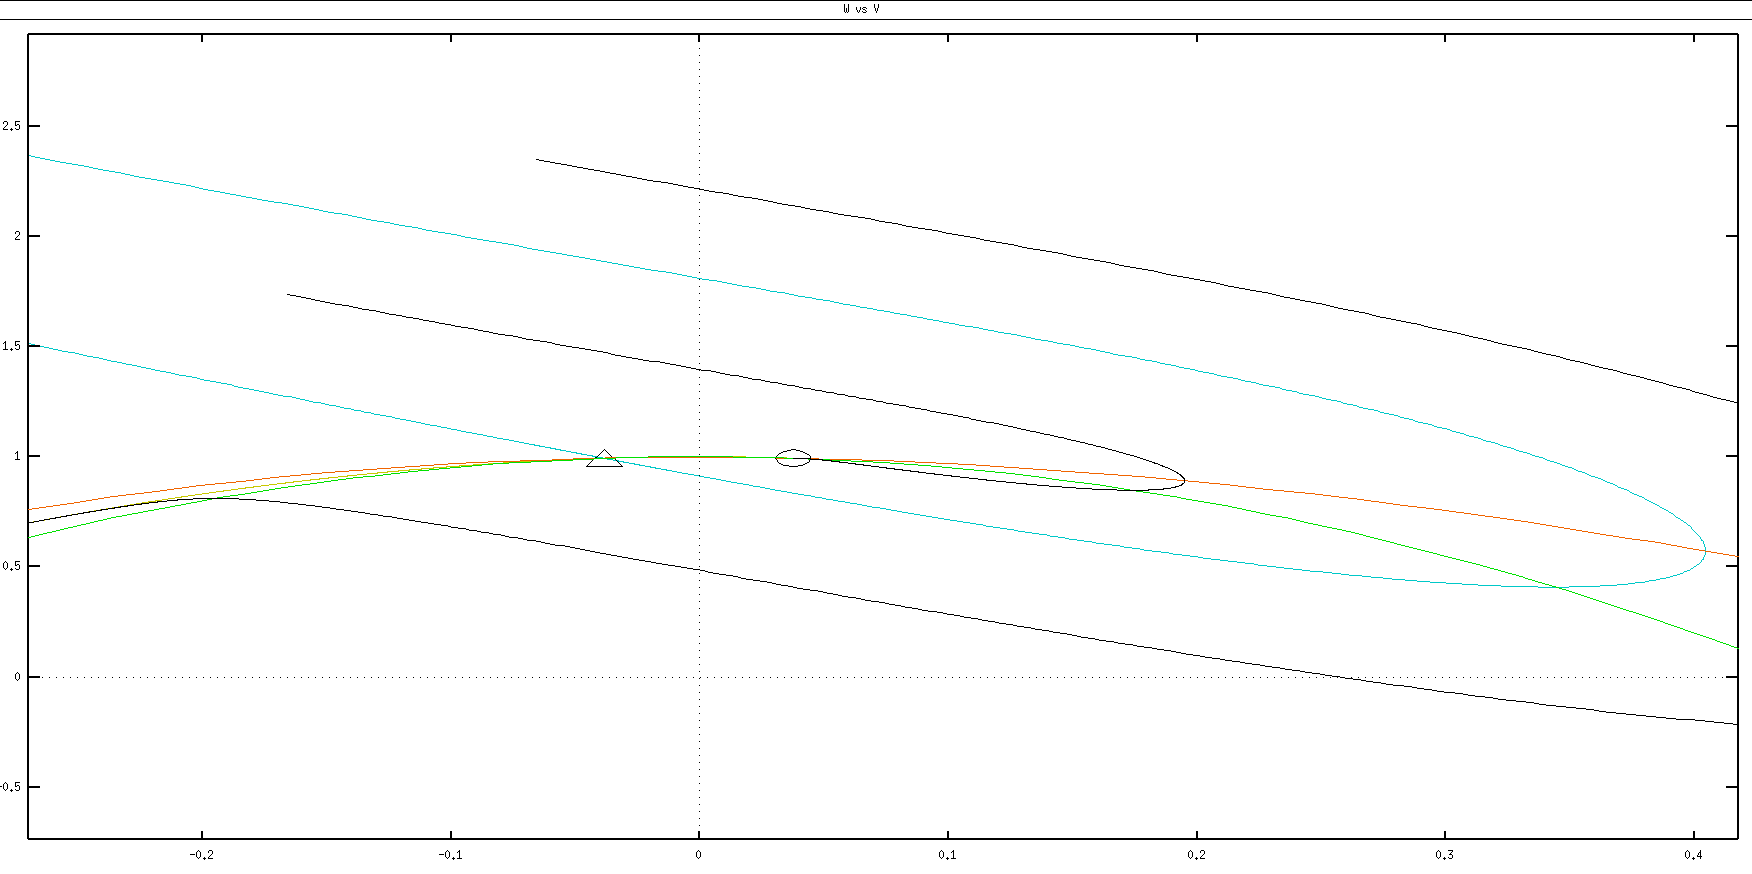
\includegraphics[ width = 0.5\textwidth]{6I-0_9971Bis.png} \\
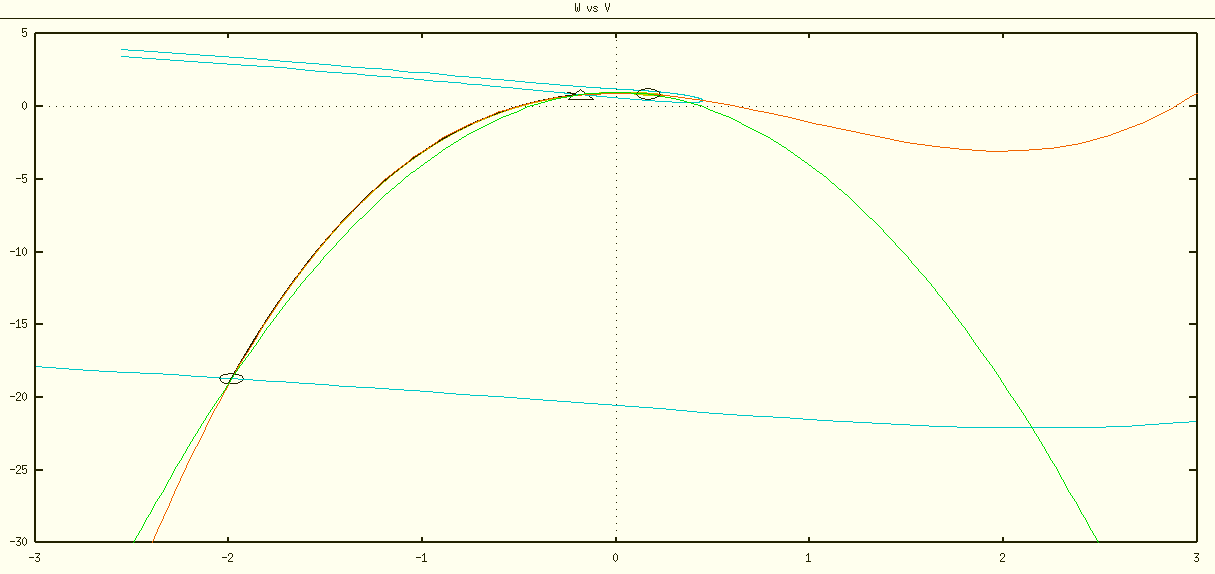
\includegraphics[ width = 0.5\textwidth]{I-0_94.png} &
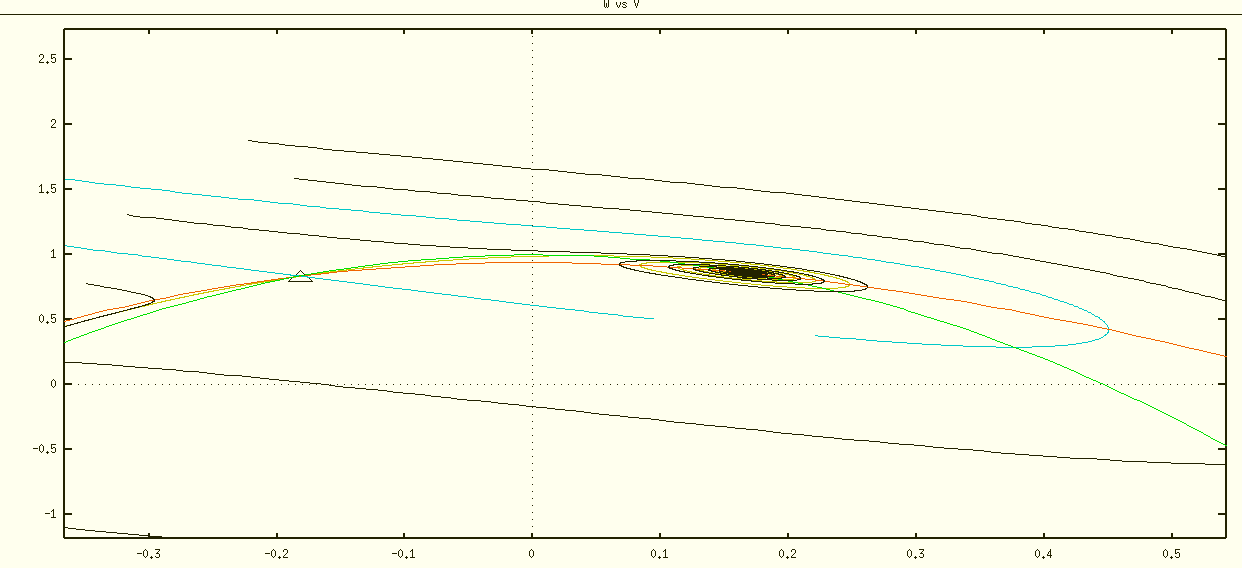
\includegraphics[ width = 0.5\textwidth]{I-0_94Bis.png} \\
\end{tabular}
\end{center}
\caption{Plan de phase $w=f(v)$. 2 attracteurs séparés par un col. En haut : pour $I_{ap} = -0.9971$ le noeud stable se transforme en foyer stable. En bas : naissance d'un cycle limite par bifurcation de Hopf. A droite, grossissement du plan de phase autour du nouvel attracteur.}
\end{figure}


\paragraph{Pour $I_{ap}$ entre -0.9265 et -0.8161}
Le foyer stable est devenu instable, et il naît un cycle limite stable par bifurcation de Hopf. Celui-ci grandit jusqu'à rencontrer le col.
\begin{figure}[H]
	\begin{center}
	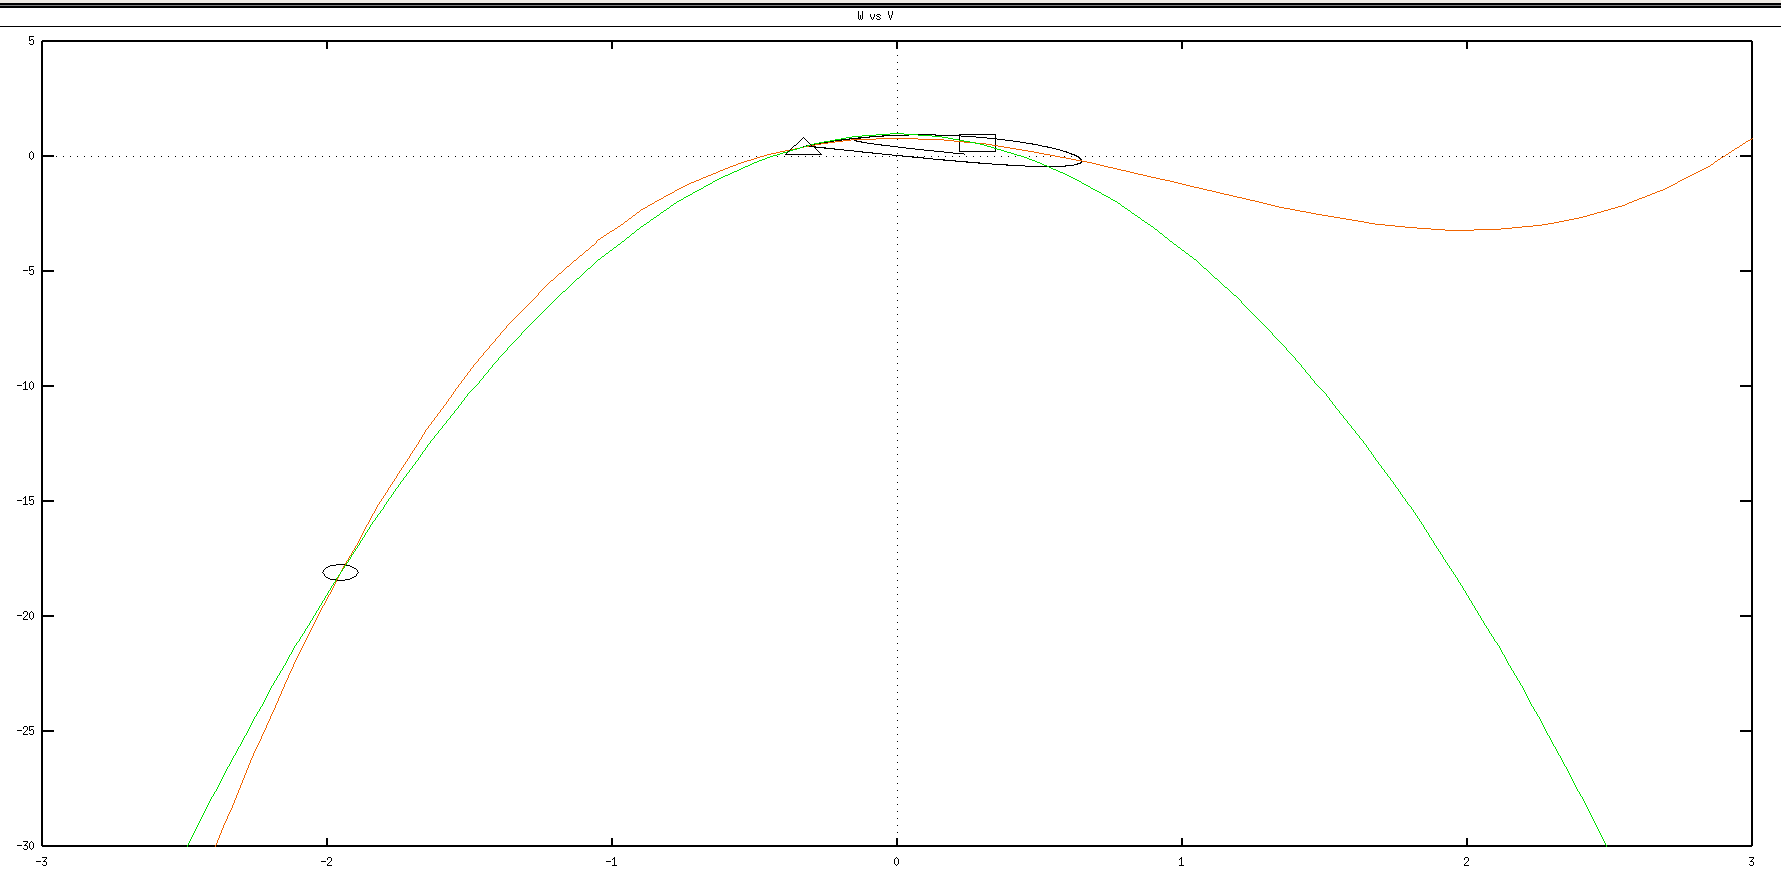
\includegraphics[ width = 0.7\textwidth]{8I-0_82.png}
	\end{center}
\caption{Plan de phase $w=f(v)$ pour $I_{ap} = -0.82$ : 1 noeud stable, un col, un foyer instable et un cycle limite stable}
\end{figure}


\paragraph{À $I_{ap} \approx -0.8161$}

La variété instable du col rejoint la variété stable en s'enroulant autour du cycle limite, et ce dernier disparaît par bifurcation homocline.

\begin{figure}[H]
\begin{center}
\begin{tabular}{p{0.5\textwidth}  p{0.5\textwidth}}
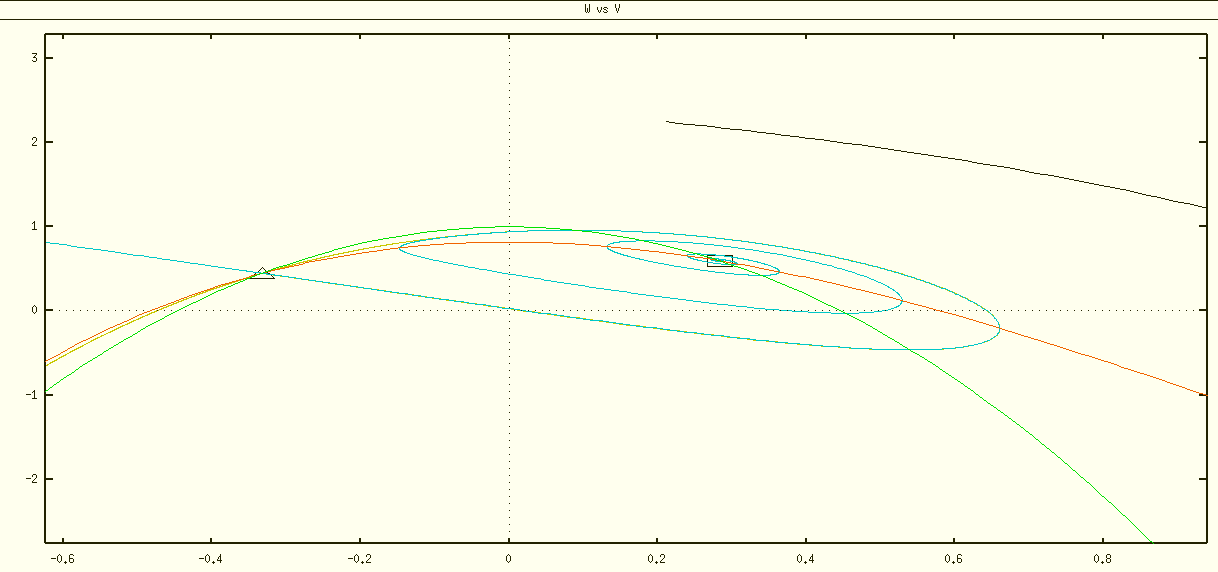
\includegraphics[ width = 0.5\textwidth]{I-0_816Bis.png} &
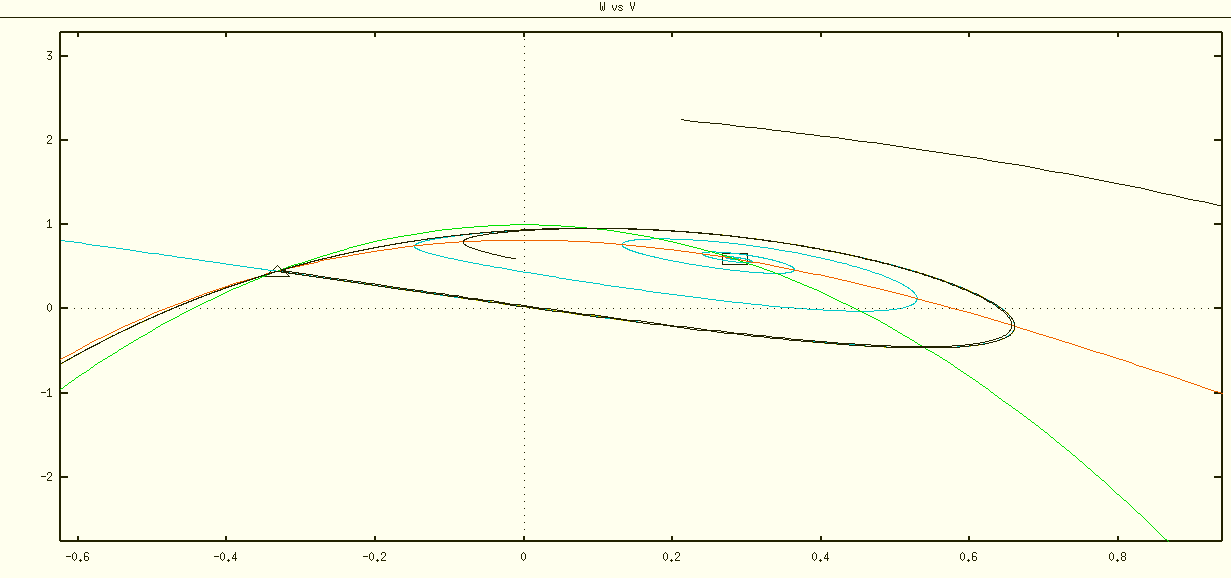
\includegraphics[ width = 0.5\textwidth]{I-0_816Ter.png}
\end{tabular}
\end{center}
\caption{Plan de phase $w=f(v)$ pour $I_{ap} = -0.816$. La variété instable du col (en bleu) s'enroule au tour du cycle limite jusqu'à rejoindre la variété stable.}
\end{figure}

\paragraph{Pour $I_{ap}$ entre -0.8161 et -0.08560}
Il y a perte de bistabilité, et du deuxième bassin d'attraction. Le seul attracteur est donc le noeud stable initial. Toute condition initiale en dehors de l'enroulement de la variété instable du col rejoint le noeud en moins d'un tour. A l'inverse, toute condition initiale à l'intérieur de l'enroulement effecteur au moins un tour dans le plan de phase autour du foyer.
\begin{figure}[H]
	\begin{center}
	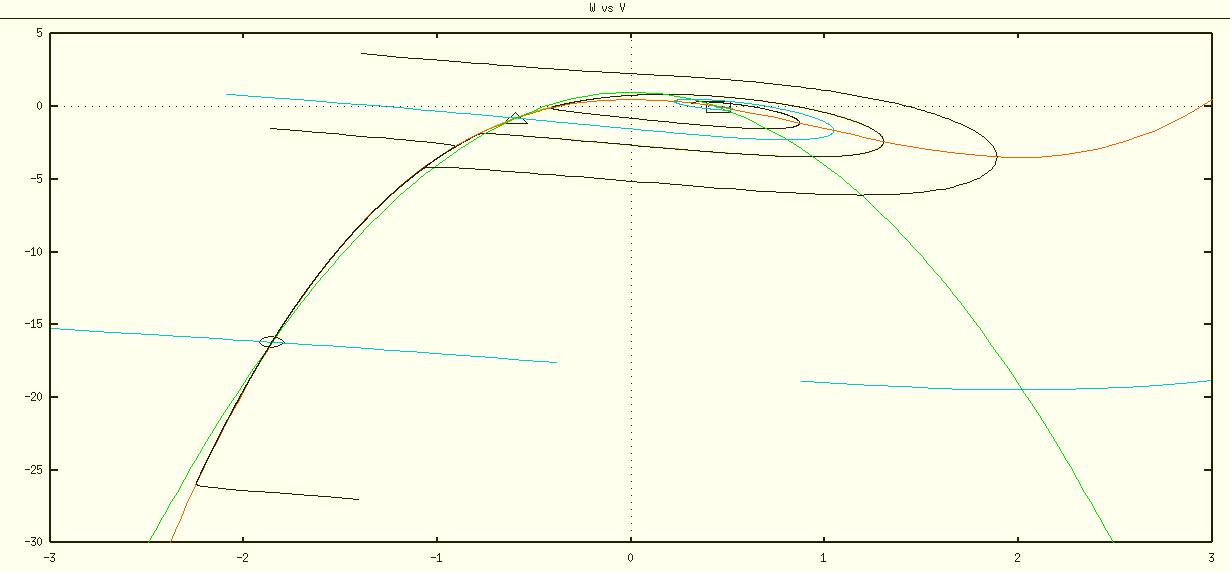
\includegraphics[ width = 0.7\textwidth]{I-0_5.png}
	\end{center}
\caption{Plan de phase $w=f(v)$ pour $I_{ap} = -0.5$ : 1 noeud stable, un col, et un foyer instable}
\end{figure}

\paragraph{À $I_{ap} \approx -0.08560$}
La variété instable du col rejoint la variété stable. Naissance d'un cycle limite par bifurcation homocline.
\begin{figure}[H]
	\begin{center}
	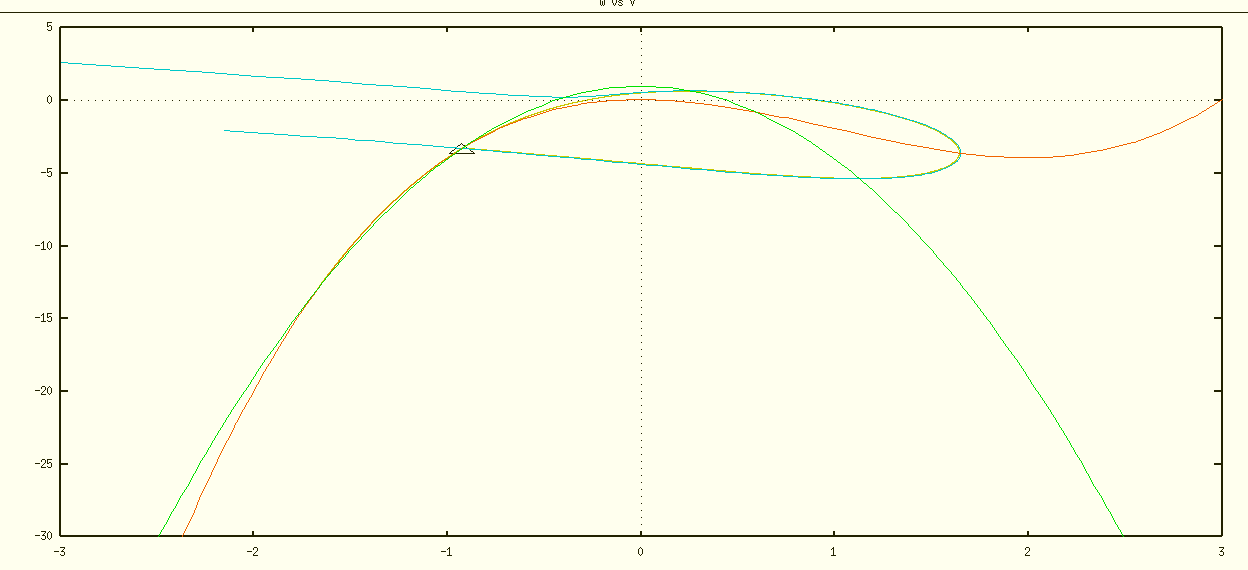
\includegraphics[width = 0.7\textwidth]{I-0_08.png}
	\end{center}
\caption{Plan de phase $w=f(v)$ pour $I_{ap} = -0.0856$. La variété instable du col, en bleu, rejoint la variété stable en s'enroulant autour d'un cycle.}
\end{figure}

\paragraph{Pour $I_{ap}$ entre -0.08560 et 0.1852}
Le cycle limite grossit, et le col se rapproche du noeud stable
\begin{figure}[H]
	\begin{center}
	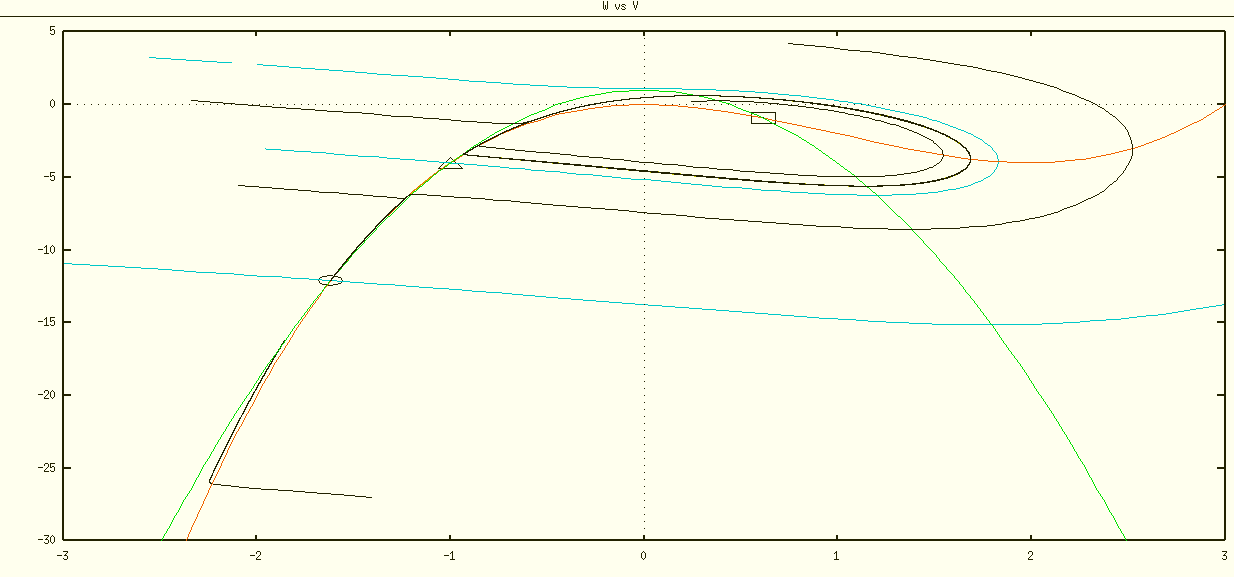
\includegraphics[width = 0.7\textwidth]{I0.png}
	\end{center}
\caption{Plan de phase $w=f(v)$ pour $I_{ap} = 0$ : 1 noeud stable, un col, un foyer instable et un cycle limite stable}
\end{figure}

\paragraph{À $I_{ap} \approx 0.1852$}
Le col est le noeud se rejoignent et disparaissent par bifurcation pli.
\begin{figure}[H]
	\begin{center}
	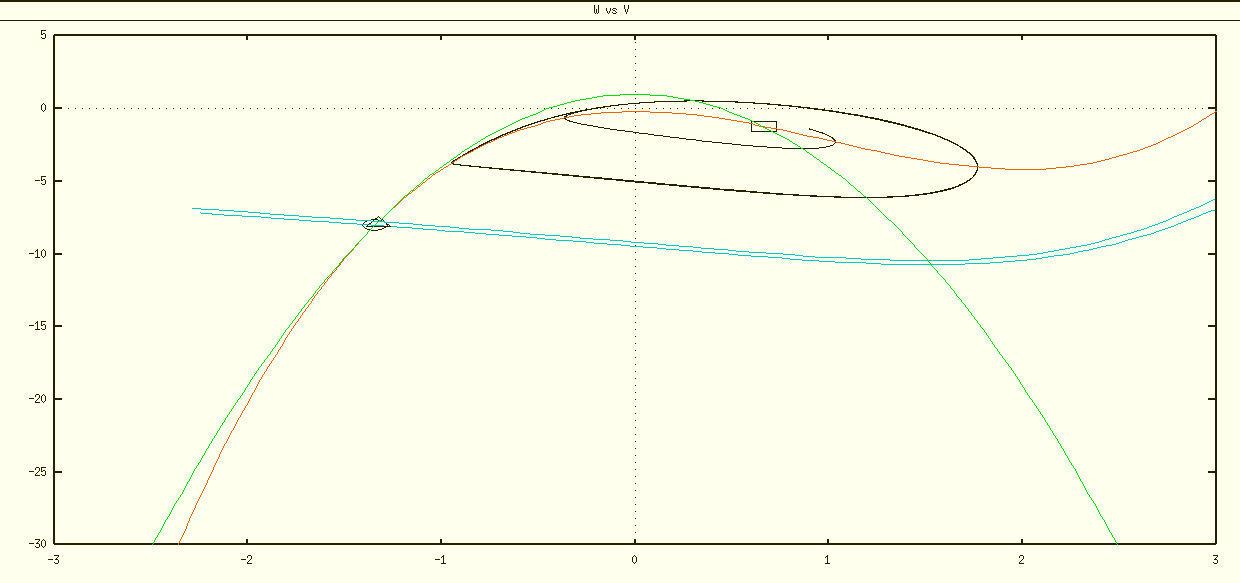
\includegraphics[width = 0.7\textwidth]{I0_185.png}
	\end{center}
\caption{Plan de phase $w=f(v)$ pour $I_{ap} = 0.185$ : 1 noeud stable, un col, un foyer instable et un cycle limite stable}
\end{figure}

\paragraph{Pour $I_{ap}$ entre 0.1852 et 10}
Le cycle limite grossit puis rétrécit. Il ne disparaît pas dans cet intervalle.
\begin{figure}[H]
\begin{center}
\begin{tabular}{p{0.5\textwidth}  p{0.5\textwidth}}
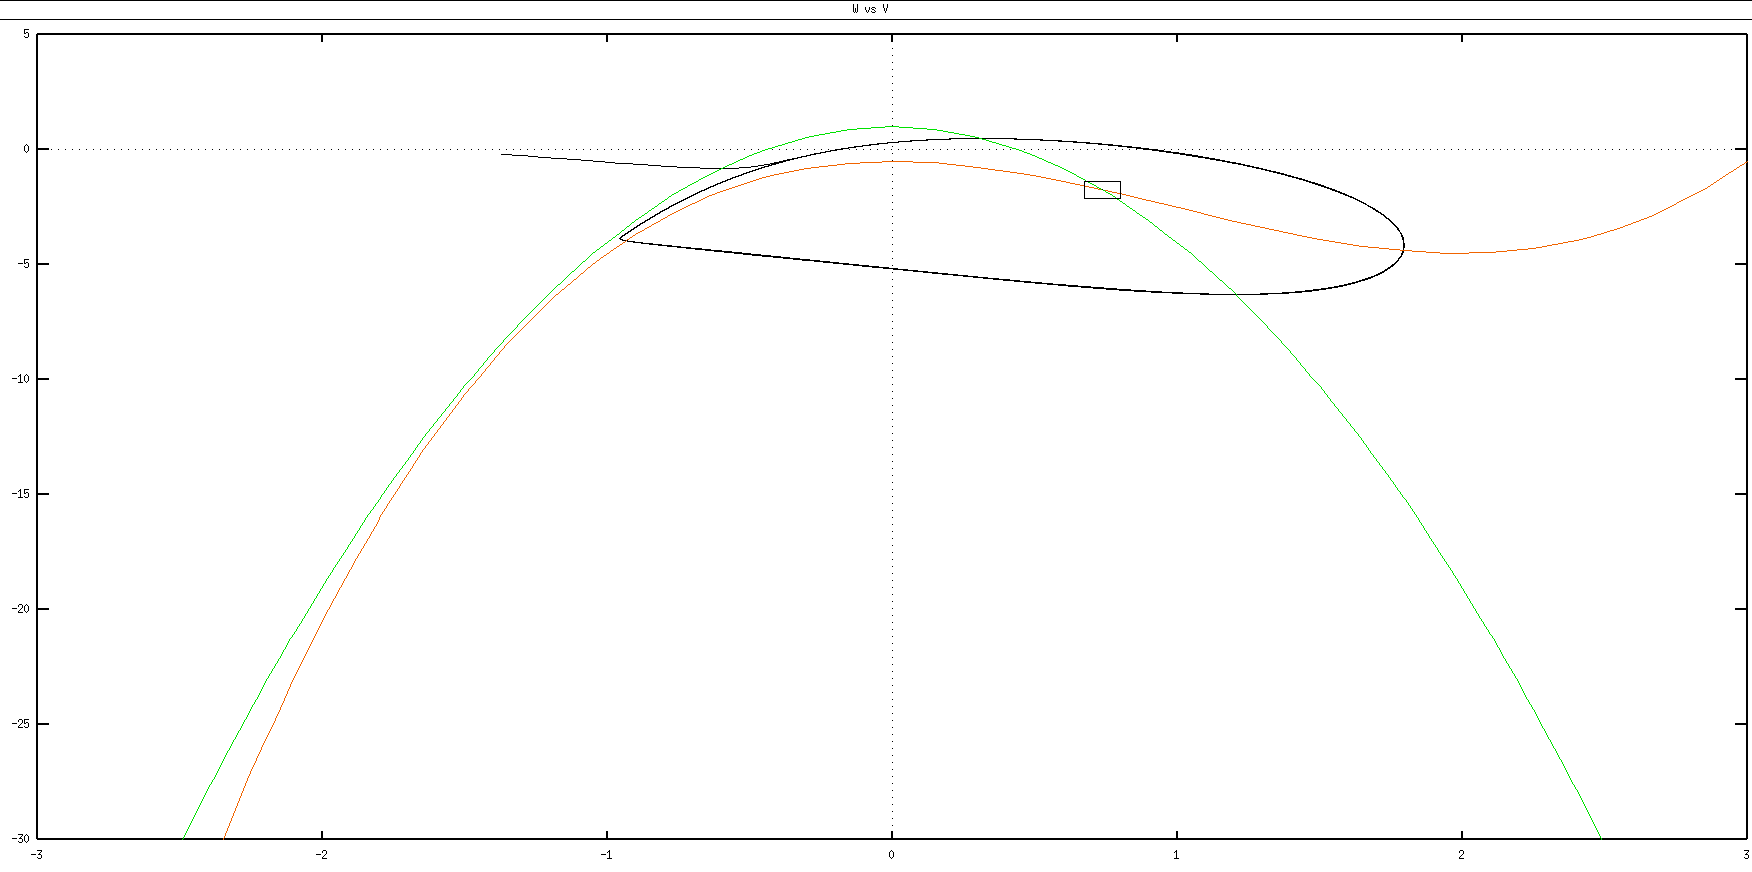
\includegraphics[ width = 0.5\textwidth]{14I0_5.png} &
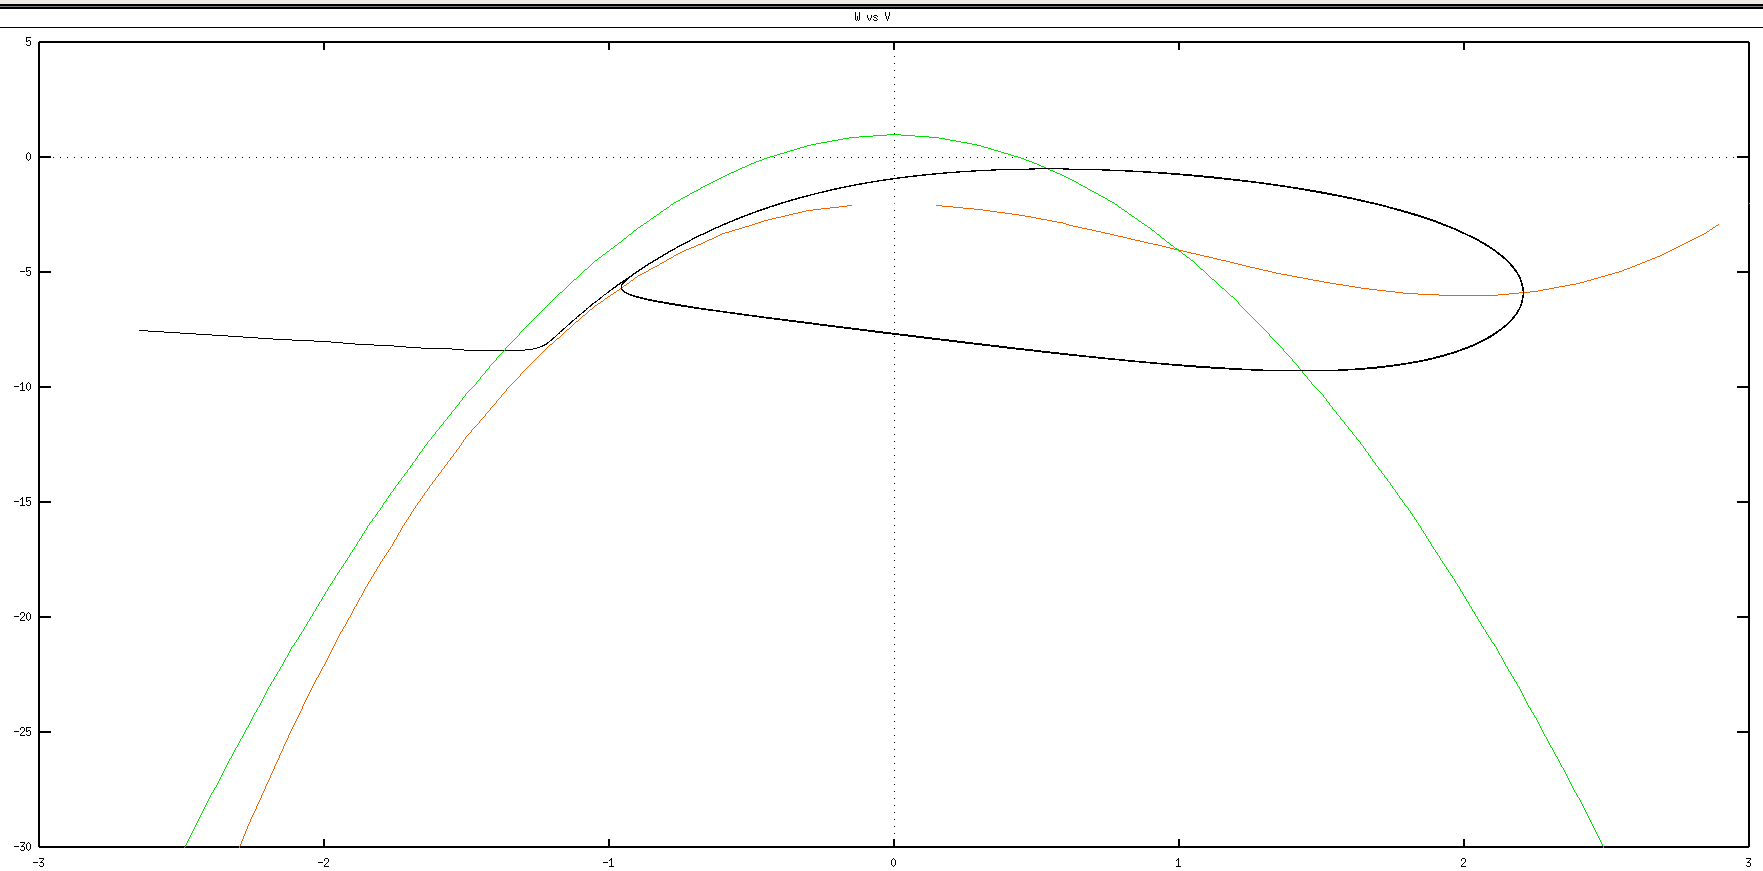
\includegraphics[ width = 0.5\textwidth]{16I2.png} \\
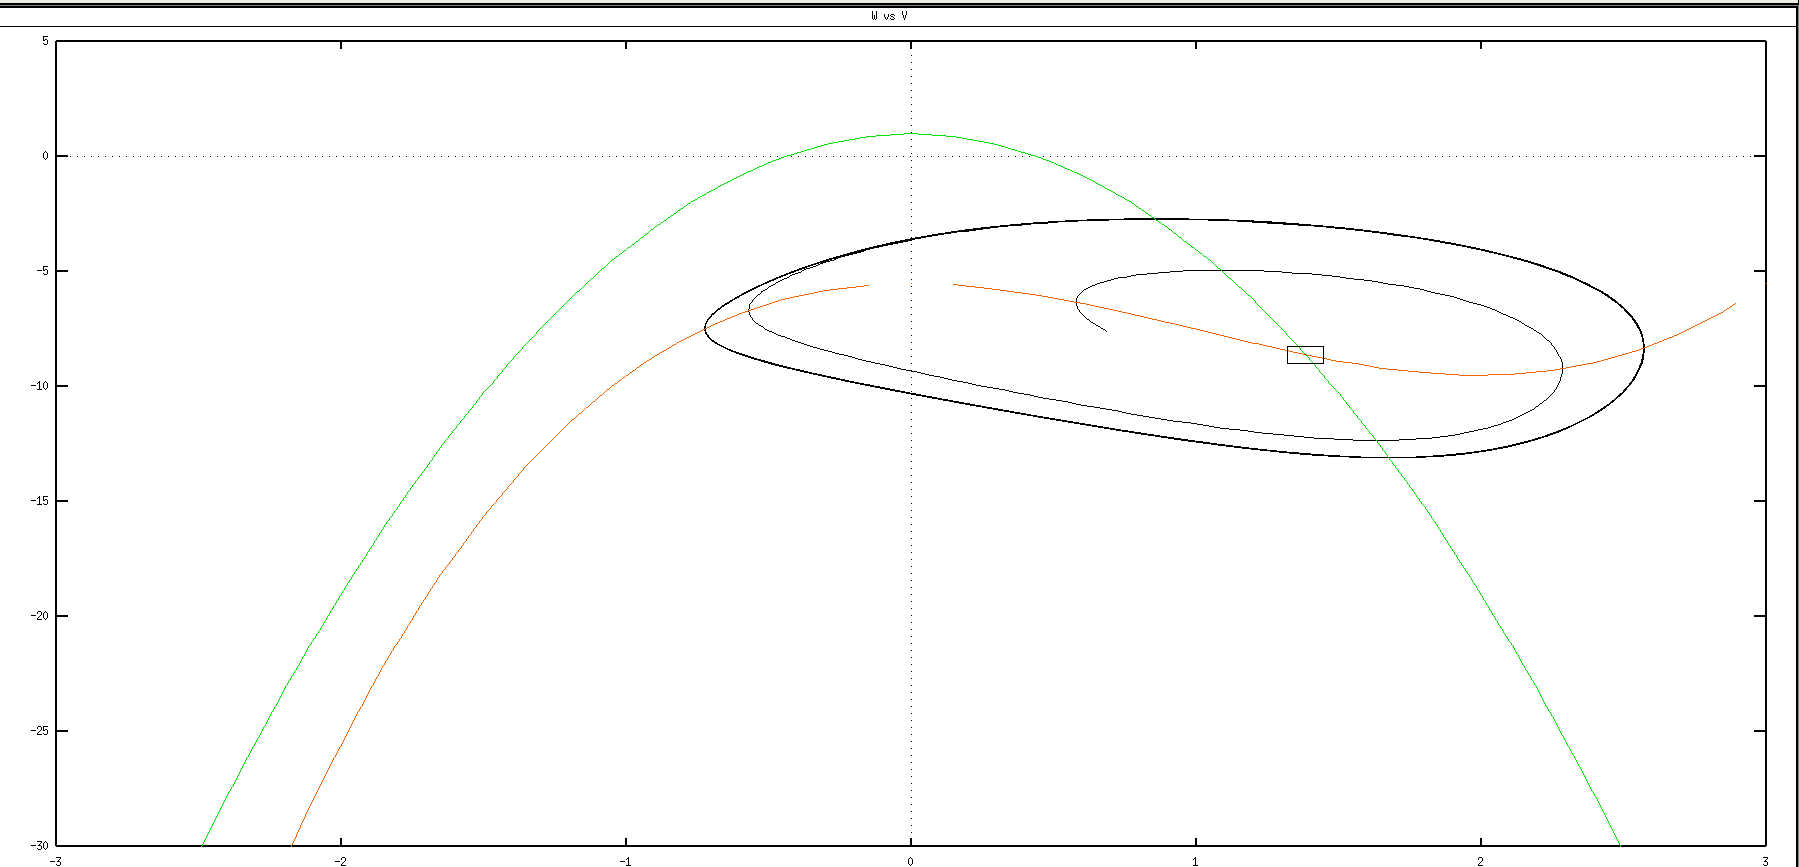
\includegraphics[ width = 0.5\textwidth]{18I5_5.png} &
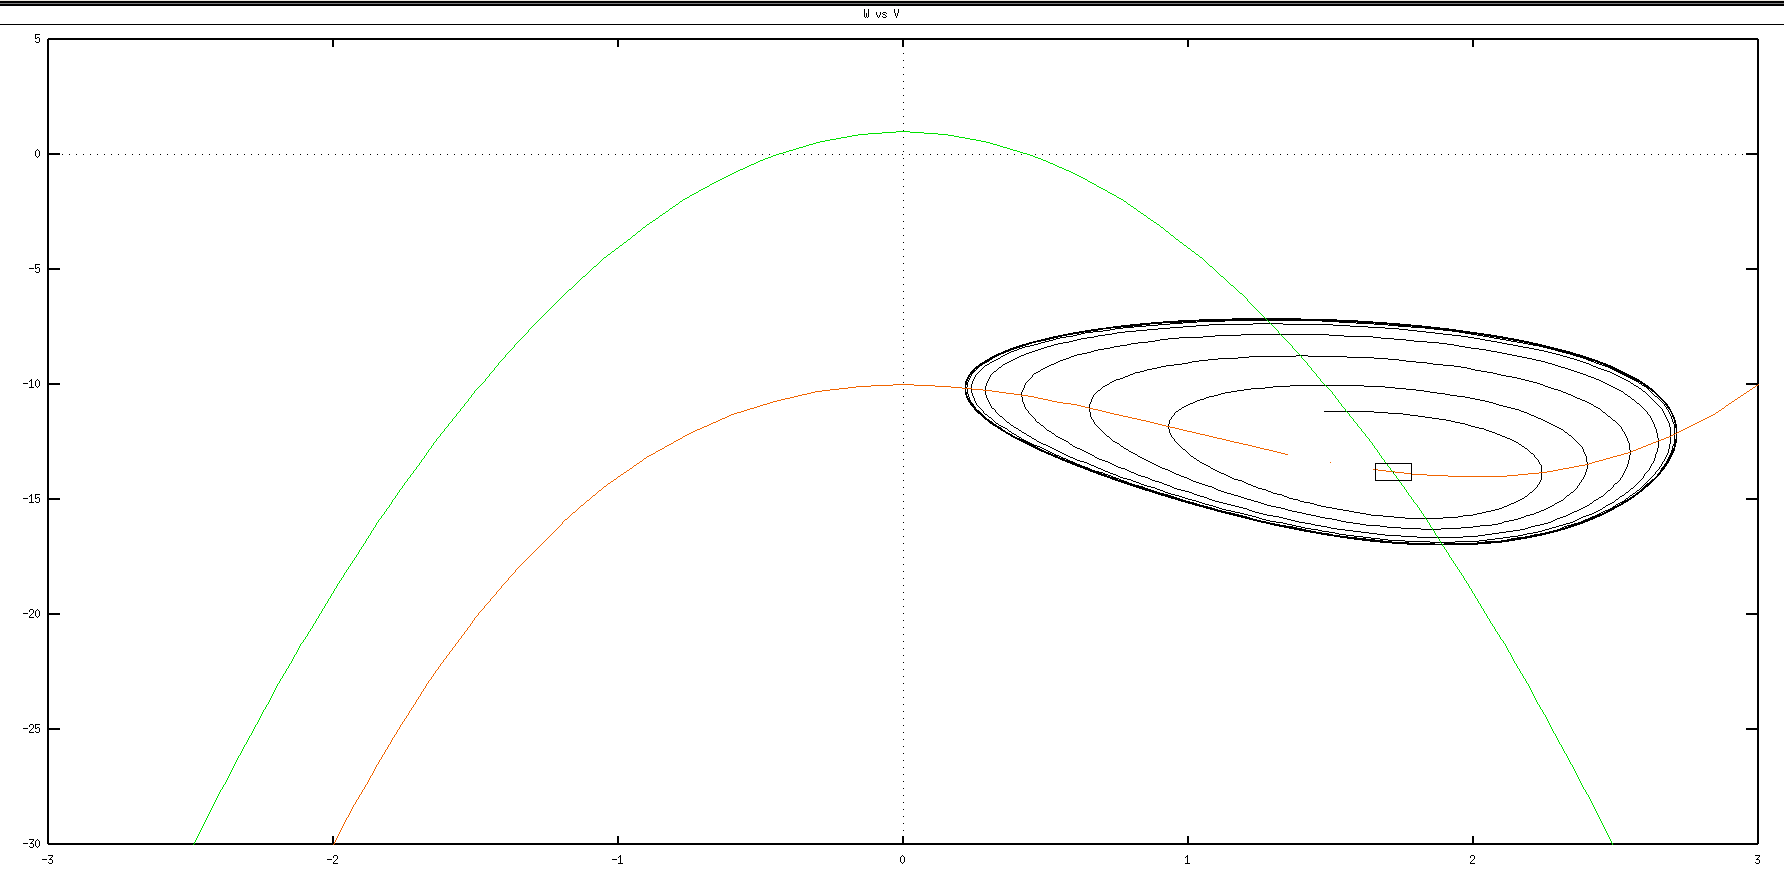
\includegraphics[ width = 0.5\textwidth]{19I10.png} \\
\end{tabular}
\end{center}
\caption{Plan de phase $w=f(v)$ pour des valeurs de $I_{ap}$ respectives de 0.5, 2, 5.5, et 10. Un seul point stationnaire, foyer instable et un seul attracteur, un cycle limite.}
\end{figure}

Le cycle limite disparait aux alentours de  $I_{ap}=11,5$, valeur pour laquelle le foyer redevient stable. Celui-ci se transforme ensuite un noeud stable pour $I_{ap}=55,26$.

\subsubsection{Résumé pour $c=1$}

\begin{tabular}{|C{4.5cm} | C{2.2cm} | C{8cm}  |}
\hline
\rowcolor{maroon}
Valeur de $I_{ap}$ & Nombre de points stat & Caractérisation des points \\
\rowcolor{maroon!10}
$I_{ap} \in [-2, -1[$ & 1 & noeud stable \\
\rowcolor{maroon!50}
$I_{ap} = -1$ & 2 & \textcolor{white}{\textbf{Bifurcation pli}} \newline noeud stable et \textbf{col-noeud} \\
\rowcolor{maroon!10}
$I_{ap} \in [-1, -0.9972[$ & 3 & noeud stable, \textbf{col} et \textbf{noeud stable} \\\hline
\rowcolor{maroon!10}
$I_{ap} \in [-0.9972, -0.9265[$ & 3 & noeud stable, col et \textbf{foyer stable} \\
\rowcolor{maroon!50}
$I_{ap} \approx -0.9265$ &
\multicolumn{2}{c|}{\textcolor{white}{\textbf{Bifurcation Hopf}}} \\
\rowcolor{maroon!10}
$I_{ap} \in [-0.9265, -0.8161[$ & 3 & noeud stable, col, \textbf{foyer instable} et \textbf{cycle limite stable} \\\hline
\rowcolor{maroon!50}
$I_{ap} \approx -0.8161$ & \multicolumn{2}{c|}{\textcolor{white}{\textbf{Bifurcation homocline}}} \\
\rowcolor{maroon!10}
$I_{ap} \in [-0.8161, -0.08560[$ & 3 & noeud stable, col et \textbf{foyer instable}\\\hline
\rowcolor{maroon!50}
$I_{ap} \approx -0.08560$ & \multicolumn{2}{c|}{\textcolor{white}{\textbf{Bifurcation Homocline}}} \\
\rowcolor{maroon!10}
$I_{ap} \in [-0.08560, 5/27[$ & 3 &  noeud stable, col, foyer instable et \textbf{cycle limite stable}\\
\rowcolor{maroon!50}
$I_{ap} = 5/27$ & 2 & \textcolor{white}{\textbf{Bifurcation pli}} \newline foyer instable, cycle limite stable et \textbf{col-noeud} \\
\rowcolor{maroon!10}
$I_{ap} \in ]5/27, 10]$ & 1 &  foyer instable et cycle limite stable\\\hline
\end{tabular}
\vspace*{0,3cm}

Le système possède des régions de bistabilité, comme présenté en figure \ref{fig_res_c_1}
\begin{itemize}
\item Pour $I_{ap} \in ]-1, -0,9262[$ avec 2 points stables,
\item Pour $I_{ap} \in ]-0,9262, -0,8161[$ avec 1 point stable et un cycle limite
\item Pour  $I_{ap} \in ] -0,008560, 5/27[$ avec 1 point stable et un cycle limite stable
\end{itemize}

\section{Système à 3D et bursting}
\subsection{Obtention du bursting}
Comme proposé dans l'article fondateur du nodèle \cite{hindmarsh1984model}, une troisième équation est introduite, transformant $I_{ap}$ en variable lente à l'aide d'un nouveau paramètre $\epsilon$.
\begin{equation}
\left\{
\begin{array}{l }
v'(t)= (w - v^3 + 3v^2 +I_{ap})/c = f(v,w) \\
w'(t) = 1 - 5 v^2 - w = g(v,w)  \\
\textcolor{blue}{I_{ap}'(t)= \epsilon (0.3 I_{ap} -1 -v)}
\end{array}
\right.
\label{sys_burst}
\end{equation}
Dans ce nouveau système \ref{sys_burst}, $(v, w)$ forme un sous-système rapide, qui a été etudié. Que ce soit pour $c=2$ ou $c=1$, il présente des zones de multistabilité.

De plus, si on considère comme établit le régime stationnaire c'est-à-dire que $v$ a atteint un état stationnaire $v_0$ alors on peut utiliser l'équation \ref{Stat} pour la nouvelle équation introduite dans le système :
$$
I'_{ap}(t) = \epsilon(0.9v_0^3+0.6v_0^2-v_0-1.3)
$$
Il y a trois racines réelles de $I'_{ap} = 0$ :
$\left\{
\begin{array}{rl}
v_1 &\approx -2.64087\\
v_2 &\approx -1\\
v_3 &\approx 1.64087\\
\end{array}
\right.$
Ce qui permet le signe de $I'_{ap}$ :
\begin{center}
	\begin{tabular}{|L{2.2cm} | C{1.5cm} | C{1.5cm} | C{1.5cm} |C{1.5cm}|C{1.5cm}|C{1.5cm}|C{1.5cm}|}
	\hline
	\multicolumn{8}{|c|}{$c \in [1, 2]$}
	\\\hline
	Valeur de $v$ & $v < -2.64$ & $v = -2.64$ & $ -2.64 < v < -1$ & $v = -1$ & $-1 < v < 1.64$ & $v=1.64$ & $v > 1.64$ \\
	 \hline
	$I'_{ap}$ & -- & 0 & + & 0 & -- & 0 & +\\ \hline
	\end{tabular}
\end{center}

\printbibliography

\end{document}
